
\title{Recap Computer System Security (02KRQOV)}
\author{Jacopo Nasi\\
        Computer Engineer\\
        Politecnico di Torino}
\date{I Period - 2018/2019\\\bigskip\bigskip\today}

\documentclass[12pt]{article}
\usepackage[utf8]{inputenc}
\usepackage[english]{babel}
\usepackage{geometry}
\usepackage{indentfirst} % First line indent
\usepackage{mathtools}
\usepackage{wrapfig}
\usepackage[usenames, dvipsnames]{color}
\usepackage{float}
\usepackage{amssymb}
\usepackage{ifsym}
\usepackage{listings}
\usepackage{multicol}

% Misure Documento
\geometry{ a4paper, total={170mm,257mm},left=35mm, right=35mm, top=35mm, bottom=35mm }

\begin{document}

\begin{figure}
  \centering
  
\includegraphics[width=10cm]{images/polito.pdf}
\end{figure}

\maketitle


\newpage
\tableofcontents

\newpage
{\noindent \Large \textbf{License}\bigskip}

This work is licensed under a Creative Commons Attribution-NonCommercial-ShareAlike 3.0 Unported License.\\
You are free:
\begin{itemize}
  \item \textbf{to Share}: to copy, distribute and transmit the work
  \item \textbf{to Remix}: to adapt the work
\end{itemize}
Under the following conditions:
\begin{itemize}
  \item \textbf{Attribution}: you must attribute the work in the manner specified by the author or licensor (but not in any way that suggests that they endorse you or your use of the work)
  \item \textbf{Noncommercial}: you may not use this work for commercial purposes.
  \item \textbf{Share Alike}: if you alter, transform, or build upon this work, you may distribute the resulting work only under the same or similar license to this one.
\end{itemize}

\noindent More information on the Creative Commons website (http://creativecommons.org).

\begin{figure}[h!]
  \centering
  
\includegraphics[width=3cm]{images/license.png}
\end{figure}

{\noindent \Large \textbf{Acknowledgments}\bigskip}

Questo breve riepilogo non ha alcuno scopo se non quello di agevolare lo studio di me stesso, se vi fosse di aiuto siete liberi di usarlo.\\
Le fonti su cui mi sono basato sono quelle relative al corso offerto (\textbf{Computer System Security (02KRQOV)}) dal Politecnico di Torino durante l'anno accademico 2018/2019.\\
Non mi assumo nessuna responsabilità in merito ad errori o qualsiasi altra cosa. Fatene buon uso!
\newpage

\section{Introduction Security ICT System}
\textbf{Why is securoty an important issue?} Nowadays that everything is online and connected to a world wild network, the security over the ICT system has become fundamental. A lack of the secutiry could generate lose for milions of money. Also data breach become a problem.\\
Everydays technology improve and drive innovation but security must be improved together with the innovations.\\
With the increase of the number of connected devices, the IoT (Internet of Things), security start to facing a lot of more problem, the complexity of the scenario has become really really big. From personal devices, like desktop, laptop, fridge or car, by communications networks, and to distributed services, everything must be secured!\\
\paragraph{Complexity enemy of security} based on one of the first axiom of engineering: \textit{"The more complex a syste, is, the more difficult its correctness verification will be."}. Keep a system as simple as possible is always a good idea. The KISS rules (\textbf{\textit{Keep It Simple, Stupid}}) is one of the most important rule over the system security.
\paragraph{Definition of ICT Security}

\bigskip
``It is the set of products, services, organization rules and individual behaviours that protect the ICT system of a company.\\

It has the duty to protect the resources from undesired access, guarantee the privacy of information, ensure the service operation and availability in case of unpredictable events (C.I.A. = Confidentiality, Integrity, Availability).\\

The objective is to guard the information with the same professionalism and attention as for the jewels and deposit certificates stored in a bank caveau.\\

The ICT system is the safe of our most valuable information; ICT security is the equivalent of the locks, combinations and keys required to protect it.''\\
\rightline{{\rm --- \textbf{Italian Bank}}}
\bigskip

An important part of the security study is the Risk Estimation, is a fundamental step that take in account all the assets and events to evaluate the risk of something. The flow is showed in figure \ref{fig:risk_est}:

\begin{figure}[h!]
  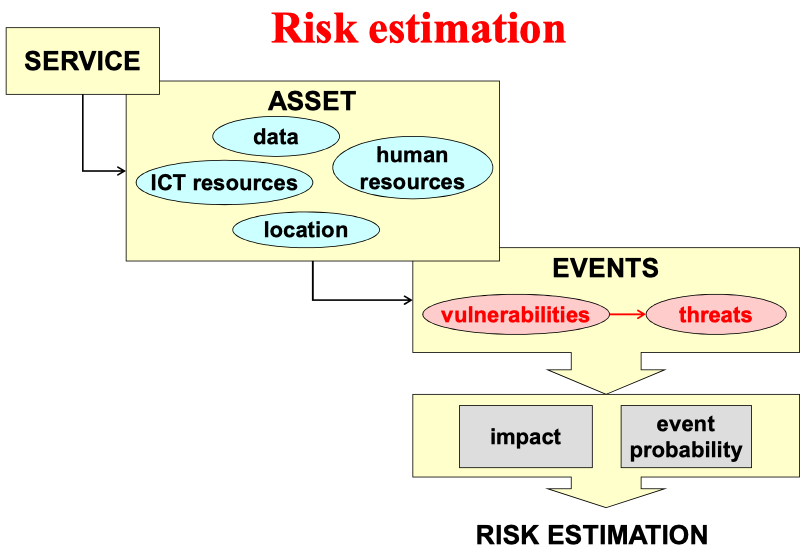
\includegraphics[width=\linewidth]{images/risk_est.png}
  \caption{Risk Estimation}
  \label{fig:risk_est}
\end{figure}

Where the assets is composed by everythings needed by a service to work, both soft and hard part, also human resources. The vulnerabilities, intrinsic of an asset, represent the weakness of it. The threats is a deliberate action, or an accidental event, that can produce the loss of a security properties exploting a vulnerability. The event is also characterized by an impact and a probability that could be high, low or other middle values.\\
Direct following of the risk estimation is the Analysis and management of security. After the evaluation of risks, is necessary to:
\begin{enumerate}
  \item Select Countermeasures
  \item Implement Countermeasures
  \item Audit (check if works)
\end{enumerate}

The security implement is not a phase of the developmente process, is part of each sigle part of it. Security can't be compute at the end of the development, it must be implement from the beginning of the process. \textbf{Security is a process, not a product!} The following figure \ref{fig:dev} show the parallel line followed by the security development.

\begin{figure}[h!]
  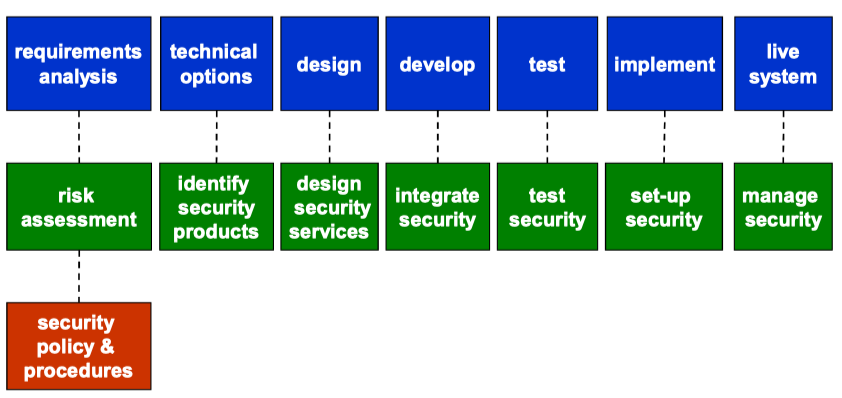
\includegraphics[width=\linewidth]{images/dev.png}
  \caption{Security Life Cycle}
  \label{fig:dev}
\end{figure}

An important definition, before speaking about security itself, is the \textbf{Window of Exposure} the represent the time when an attack could be perfomed and there are no countermeasures to avoid it. This window could potentially be infinite and this is the real problem.
The figure \ref{fig:window} show how this windows id divided in different part:

\begin{figure}[h!]
  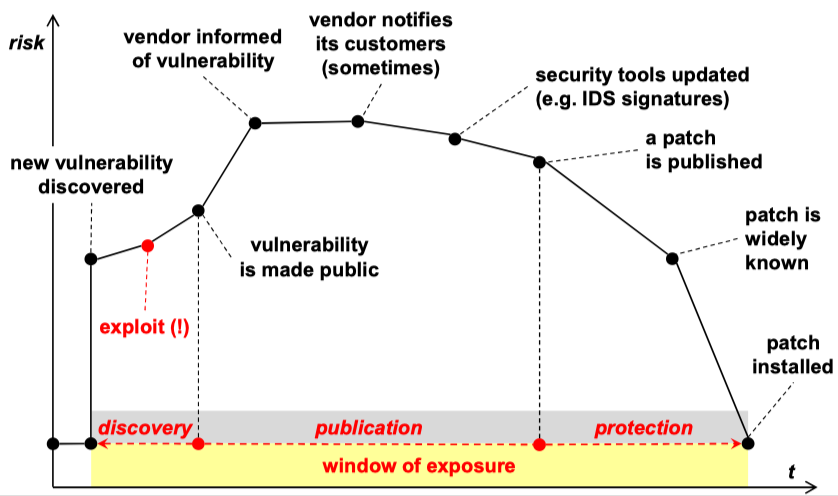
\includegraphics[width=\linewidth]{images/window.png}
  \caption{Window of Exposure}
  \label{fig:window}
\end{figure}

As already says, security is not a product but is a proccess. Computer flaws are inevitable and this is way we can't use devote our security to only secured products. The only way to effectively do business is an insecure world is to put processes in place that recognize the inheritent insecurity in the products. \textbf{The trick is to reduce your risk of exposure regardless of the products or patches}.

\paragraph{Security Principles} Here some of the most important security principles:
\begin{itemize}
  \item Security by Design
  \item Least Privilege: Only correct rights and the only few needed
  \item Need-to-know: Access to the only piece of stuff that are needed
  \item Security by Default
  \item Security in Depth: More the importance of the system, more the obstacles
\end{itemize}

\paragraph{Security Properties} The following list show the most importante properties of the security world:
\begin{itemize}
  \item Authentication (Simple/Mutual): Source (or both) must prove themself
  \item Data Origin/Authentication
  \item Authorization and Access Control
  \item Confidentiality/Privacy/Secrecy
  \item Non Repudiation: Formal proof, acceptable by a court of justice, that gives undeniable evidence of the data creator
  \item Availability
  \item Accountability
  \item Integrity: Modification, Filtering
\end{itemize}

\paragraph{Where is the enemy?} The enemy normally is supposed to be outside of our system but is not simple as it seems. The possible locations are:
\begin{itemize}
  \item Outside our organization (Firewall)
  \item Outside our organization, with exceptionn of our parters (VPN)
  \item Inside our organitazion
  \item Everywhere!
\end{itemize}
The last item is probably the more true. The distinction between internal/external and good/bad guys is no more sufficent. From the \textit{Verizon Data Breach Invetigation Report} the percentage of source of attacks is: 20\% Internal and 80\% External, probably the internal percentage is a little bit higher due to the fact that Verizon is a provider and can't show the internal side so much.

\paragraph{Basic Problems} There are some basic problem for security:
\begin{itemize}
  \item Networks are insecure:
  \begin{itemize}
    \item Clear communications
    \item LAN use broadcast
    \item Not E2E geographical connections
  \end{itemize}
  \item Weak user Authentication
  \item No server Authentication
  \item \textbf{Software with bugs!}
\end{itemize}

\paragraph{Classes of Attacks} Some of the most common type of attacks:
\begin{itemize}
  \item IP Spoofing / Shadow Server
  \item Packet Sniffing
  \item Connection Hijacking / Data Spoofing
  \item Denial-of-Service (Distributed DoS)
\end{itemize}
The \textbf{IP Spoofig}, or source address spoofing, is forginng the sourcce network address, typically performed at LV3 (IP), but also at LV2 can be performed. The typical attacks are: Data Forging and unauthorized access to systems.\\
The \textbf{Packet Spoofing} it reads the packet addresses to another network node, it easy to do in LAN or at the switching nodes. It allows to intercept password, data and other stuffs.\\
The \textbf{Denial-of-Service (DoS)} it keeps a host busy so that it can't provide its services. There are a lots of examples: mail/log saturation, ping flooding, SYN attacks. The main problem of this kind of attacks is that there are no countermeasures. The \textbf{Distributed DoS} are similar to the previous one but perfomed by a greater number of hosts (botnet), controlled by a master. The power is the same of a normal DoS multiplied by the number of deamons of the botnet. There are also some techniques to improve the attack like using a reflector to hide the attacker's track. One of the more important DDoS was performed agains Yahoo! during Feb 2000.\\
The \textbf{Shadow Server} is a technique that host that manage the attacks show itself (to victims) as a service provider without having the right to do so. It provide a "wrong" serice to victims, like bank sites or other stuffs.\\
\textbf{Connection Hijacking / MITM}, AKA Data Spoofing, is performed when attacker takes control of a communicatio channel to insert, delete, or manipulate traffics. It can edit data is all forms, and change the messages of the communications. Another similar for is the \textbf{Trojan / MITB}, it used the fact that network channels are more protected, but users terminals not. The behaviour is to install a keylogger to store everything. It could be also passed via browser extension.\\
The are other application-leve problems:
\begin{itemize}
  \item Buffer Overflow
  \item Cookies
  \item Clear password in DB
  \item "invent" a protection system
\end{itemize}
We make now some clearance about name of malwares:
\begin{itemize}
  \item Virus: Damage the target and replicate itself, propagated by humans (require complicity)
  \item Worm: Damage target because replications (resource saturation)
  \item Trojan: Malware vector
  \item Backdoor: Unauthorized access point
  \item Rootkit: Privileged access tools, hidden and stealth
  \item Ransomware: Make hosts unreadable (can be also silent)
\end{itemize}

\paragraph{Non technological problems} Prorably the greatest majority of the problems and leaks come from here! The are some basic problems: due to low awareness, mistakes, tendency to trust and other facts the major cause of leaks are humans.\\
The \textbf{Social Engineering} are sets of techniques used to asks the involutary user's partecipatio to the attack action, usually the naïve users are targeted (e.g. \textit{“do change immediately your password with the following one, because your PC is under attack”}), also experienced users are targeted (e.g. by copying an authentic mail but changing its attachment or URL).\\
One of the most used technique is the \textbf{Phishing} (~fishing) where the attacker try to stole information (fishing) from the target (fish), it can be achieved, for example, by showing acquaintance with the company’s procedures, habits and personnel helps in gaining trust and make the target lower his defences. Is often performed by using fake mail, SMS or IM. The normal procedures works by attarcting the fish in a shadow server where it will leave of the sensitive informations or persuade to install plugins or other stuffs. Two variants exist, \textbf{spear phishing} (include several personal data to disguise the fake message as a good one, e.g. mail address, name of Dept/Office, phone no.) or \textbf{whailing} (targeted to VIP such as CEO or CIO).
The \textbf{Pharming} is a set of several techniques to re-direct a user towards a shadow server, chaging the hosts file, nameserver, poisoning cache of DNS. Some important examples of this techniques are T.J.Maxx attack, Transformed3 phishing or Stuxnet.\\
The typical path of attackers is showed in figure \ref{fig:killchain}.

\begin{figure}[h!]
  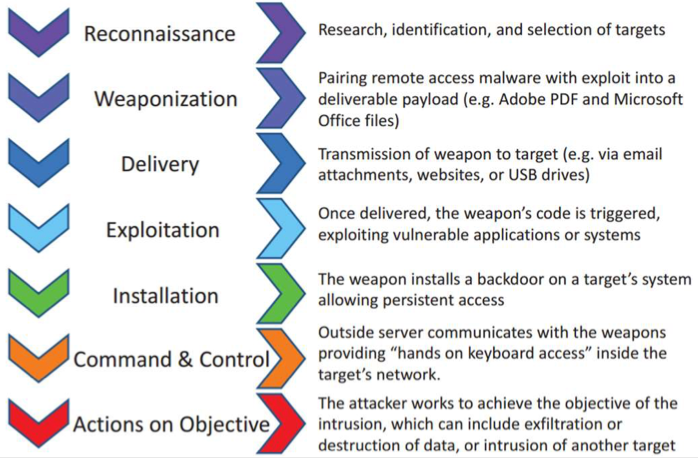
\includegraphics[width=\linewidth]{images/killchain.png}
  \caption{Cyber (intrusion) Kill Chain}
  \label{fig:killchain}
\end{figure}

From this brief introduction we can define he three pillars of security:
\begin{figure}[H]
  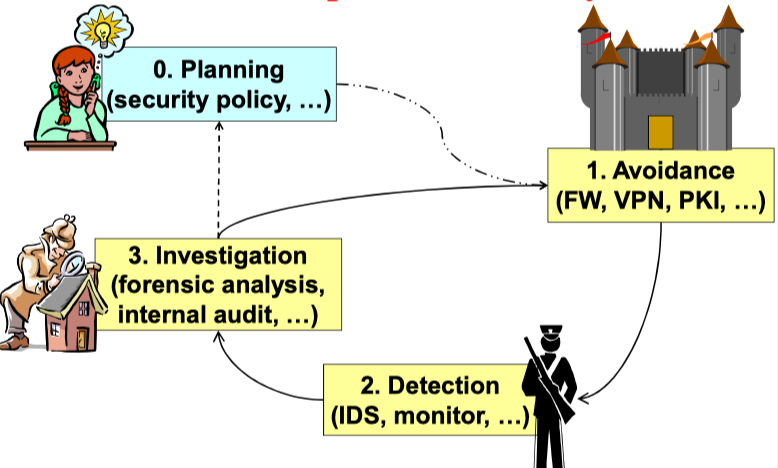
\includegraphics[width=\linewidth]{images/pillars.png}
  \caption{Pillars of Security}
  \label{fig:pillars}
\end{figure}
and we can define the main figures:
\begin{itemize}
  \item Hacker: Good and skilled
  \item Cracker: Bad but skilled
  \item Script Kiddie: Bad but NOT skilled
  \item Wannabe Lamer: Not good at all
\end{itemize}
%--------------------------------
%         END SLIDE 1           |
%--------------------------------

\section{Basic of ICT security}
\subsection{Cryptography Introduction}
The basic principles of Cryptography are showed in the following figure
\begin{figure}[H]
  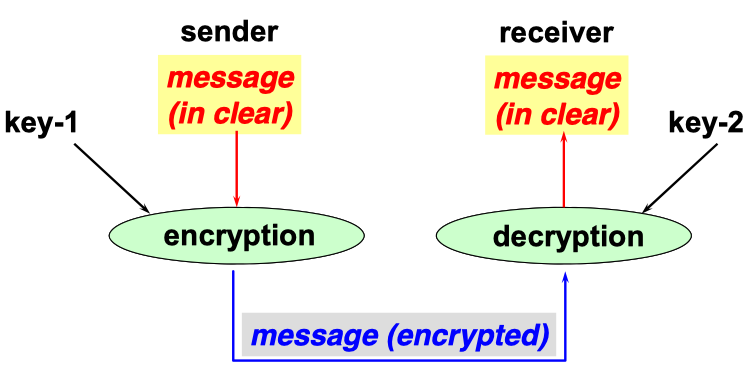
\includegraphics[width=\linewidth]{images/crypt.png}
  \caption{Cryptography flow}
  \label{fig:crypt}
\end{figure}
Some important terminology. The message in clear is called:
\begin{itemize}
  \item Cleartext or plaintext
  \item Refer with \textbf{P}
\end{itemize}
Instead the encrypted message:
\begin{itemize}
  \item Ciphertext
  \item Refer with \textbf{C}
\end{itemize}

Some principles of Cryptography, written by Kerchoffs, are:
If the keys:
\begin{itemize}
  \item Are kept secret
  \item Are managed only by trusted systems
  \item Are of adeguate lenght
\end{itemize}
then...
\begin{itemize}
  \item it has no importance that the ecryption and decryption algorithms are kept secret
  \item on the contrary it is better to make the algorithms public so that they can be widely analysed and their possible weaknesses identified
\end{itemize}
In computer system STO (Security Through Obscurity) is not good.\\
An important operator of this world is the XOR function that is the ideal confusion operator, because it not change the probability. Is also a primitive operation present in all CPUs.

\subsection{Symmetric Cryptography}
Are all the algorithms based on a secret key shared between sender and receiver, used for encrypt and decrypt. Figure \ref{fig:symm} show the general flow of this kind of algorithms. The advantage are low computational cost, in fact is used for data encryption.\\
\begin{itemize}
  \item $C = enc(K, P)$
  \item $P = dec(K, C) = enc^{-1}(K, C)$
\end{itemize}
One of the main problem is \textit{"How to share (securely) the secret key among sender and receiver?"}. T
\begin{figure}[H]
  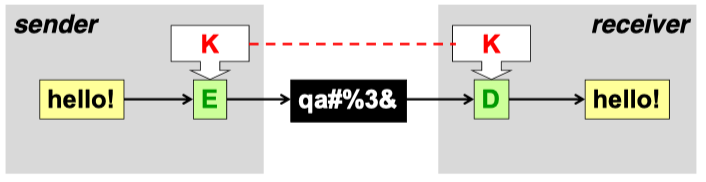
\includegraphics[width=\linewidth]{images/symm.png}
  \caption{Symmetric General flow}
  \label{fig:symm}
\end{figure}
There is not a confirmation of correct decryption, is up to the user to understand if the result is correct or not, in any case a result is provided with any key.\\

\paragraph{DES} (Data Encryption Standard) one of the first used by US government. Is now obsolete, is based on a key of 64 bits, composed by:
\begin{itemize}
  \item Key: 56 bits
  \item Parity: 8 bits
\end{itemize}
This means that the actual bit of resistence is 56. It's based on 64 bits of data blocks. It is also designed to be efficent in hardware with poor performance, the flow is:
\begin{enumerate}
  \item XOR
  \item Shift
  \item Permutation (not so good performance)
\end{enumerate}

\paragraph{3DES} is the triple repeted application of DES, it used two of three 56 bits keys. Is different from passe to a keys long 56*3 because the key lenght will not match with that number of bits. It can be computed in two ways:
\begin{itemize}
  \item 2 Keys: $C = enc(K_1, dec(K_2, enc(K_1, P)))$
  \item 3 Keys: $C = enc(K_3, dec(K_2, enc(K_1, P)))$
\end{itemize}
The central step of decryption is made to generated mess.\\
An important issue of the encryption is the doubling of an algorithms. Double application of encryption algorithms is subject to a know-plaintext attack named \textbf{meet-in-the-middle} which allows to decrypt data with at most $2^N+1$ attempts (if the keys are N-bits long). Thus the double version is never used, it double the computation time and increase they key lenght of only one bit. The formulas are:
\begin{itemize}
  \item [] $C = enc(K2, enc(K1, P))$
  \item [] $dec(C, K2) = dec(K2, enc(K2, enc(K1, P)))$
  \item [] $dec(C, K2) = enc(K1, P)$
\end{itemize}
The attacker can compute ENC(K1, P) for all values of K1 and DEC(K2, C) for all possible values of K2, and add only 1 bit of strenght for 2 keys of the same size.

\paragraph{IDEA} International Data Encryption Algorithm it was patented but with low royalty, developed for 16 bits architectures. It use a 128 bits key and 64 bits of data block, it's famous because is used in PGP. The operation used are:
\begin{itemize}
  \item XOR
  \item Addition Modulo 16
  \item Multiplication Modulo $2^{16}+1$
\end{itemize}

\paragraph{RC2, RC4} other algorithms developed by Ron Rivest (Ron's Code), they are algorithm proprietary of RSA but not patented, 3 to 10 times faster than DES. RC2 is a block algorithm, RC4 is a stream one. They are using a variable length key.

\paragraph{Application of block algorithms} applying these algorithm over data of size different from the block size require a little effort. When the data size is greater that the algorithm's block size:
\begin{itemize}
  \item ECB (Electronic Code Block)
  \item CBC (Cipher Block Chaining)
\end{itemize}
In the other case:
\begin{itemize}
  \item Padding
  \item CFB (Chiper FeedBack), OFB (Output FeedBack)
  \item CTR (Counter Mode)
\end{itemize}

The frist solution \textbf{ECB} is a bad idea, it based on the division of the data in chunks with the same size of a block, by encrypting them with a K (key), the formula is: $C_i = enc(K, P_i)$. The problems of this solution are:
\begin{itemize}
  \item Swapping of two blocks of cipher goes undetected
  \item Identical blocks generated identical cipher texts hence it is vulnerable to \textit{know-plaintext} attacks. (Word example)
\end{itemize}
These are the main reason to avoid the use of this solution for big data. The decryption is made by reversing the process. The figure \ref{fig:ecb} show the process.
\begin{figure}[H]
  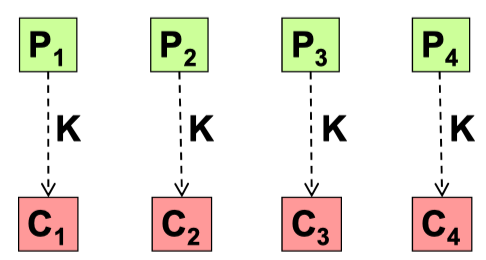
\includegraphics[width=\linewidth]{images/ecb.png}
  \caption{ECB}
  \label{fig:ecb}
\end{figure}
The solution of \textbf{CBC} [figure \ref{fig:enc_cbc}] is more secure, by using an IV (Initialization Vector), it encrypt the block by XORing it with the previous block and with the key, this avoid the problem of the \textit{know-plainntext}, because same text in different position will generate different encrypted text. The IV is added for increasing the difficulties of decryption. The formula is the following:
\begin{center}
  $C_i = enc(K, P_i \oplus C_{i-1})$
\end{center}
The decryption require the Initialization Vector ($C_{0}$), the formula is the revert the process by the following formula:
\begin{center}
  $P_i = dec(K, C_i) \oplus C_{i-1}$
\end{center}

\begin{figure}[H]
  \centering
  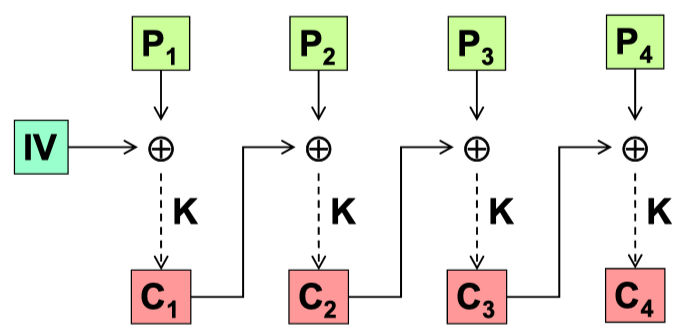
\includegraphics[width=\linewidth]{images/enc_cbc.png}
  \caption{CBC Encryption}
  \label{fig:enc_cbc}
\end{figure}

When the data is shorted than the block size, a \textbf{padding} (or aligning, filling) is required. It consist by adding some data at the end to completely fill the block. The are several techniques used for padding:
\begin{itemize}
  \item If the length is know: 0x00 bytes
  \item Original DES: 1 bit followed by 0
  \item One byte 128 (0x80) followed by null 0x00
  \item Last byte value equal to length of padding
\end{itemize}
 The are also some techniques with explicit length for padding:
 \begin{itemize}
   \item (SSL/TLS) bytes with value L
   \item (SSH2) random bytes
   \item (IPsec/ESP) progressive numbers
 \end{itemize}

Padding is typically applied to large data, on the last fragment resulting from the division in blocks (ECB or CBC), for $|D| < |B|$ we prefer ad hoc techniques like CFB, OFB or CTR. Another important note is that, even if the plaintext is an exact multiple of the block, padding must be added anyhow to avoid errors in the interpretation of the last block.\\

\textbf{CTS} (CipherText Stealing) permits to use block algorithms without padding:
\begin{itemize}
  \item Last (partial) block filled with bytes from the second-to-last block
  \item These bytes are removed from the second-to-last block (which become partial)
  \item After encryption, exchange the position of the last and second-to-last blocks.
\end{itemize}
 The figure shows better the solution algorithm:
\begin{figure}[H]
   \centering
   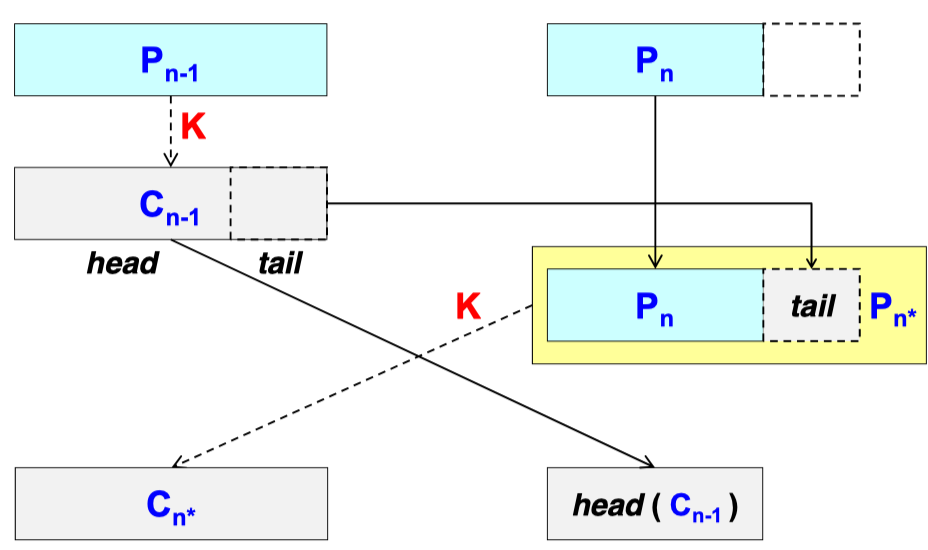
\includegraphics[width=\linewidth]{images/cts.png}
   \caption{CTS with ECB Encryption}
   \label{fig:cts}
\end{figure}
This technique is useful when we cannot increase the size of the data after the encryption. The tail, store, after the encryption in the second-to-last block is encrypted 2 times and it requires 2 decryption.\\
The \textbf{CRT} (Counter mode), really used, uses a block algorithm to cipher N bits at a time. It require:
\begin{itemize}
  \item \textbf{NONCE} = Number used ONCE
  \item counter
\end{itemize}
The flow is showed in the following figure \ref{fig:crt}:
\begin{figure}[H]
   \centering
   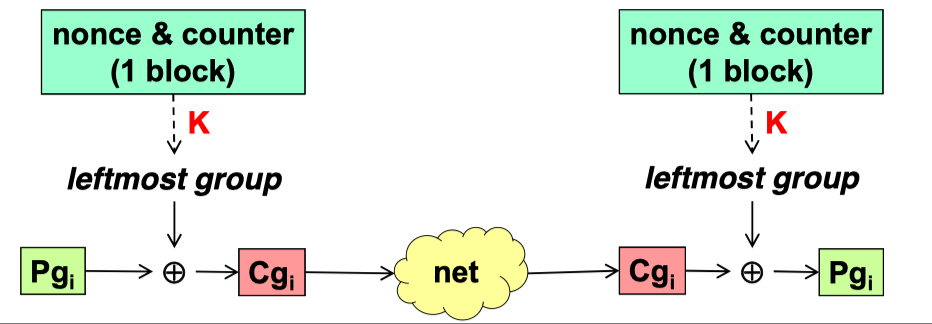
\includegraphics[width=\linewidth]{images/crt.png}
   \caption{CRT flow}
   \label{fig:crt}
\end{figure}

\paragraph{Symmetric Stream Algorithms} this kind of algorithms not require to separate datas in blocks. They operate over one bit/byte at the time. The ideal algorithms require a key which is as long as the message to protect, of course this is not possible. The real algorithms use pseudo-random key generators, synchronized between the sender and receiver, some examples are RC4 and SEAL. The idea is show in figure
\begin{figure}[H]
   \centering
   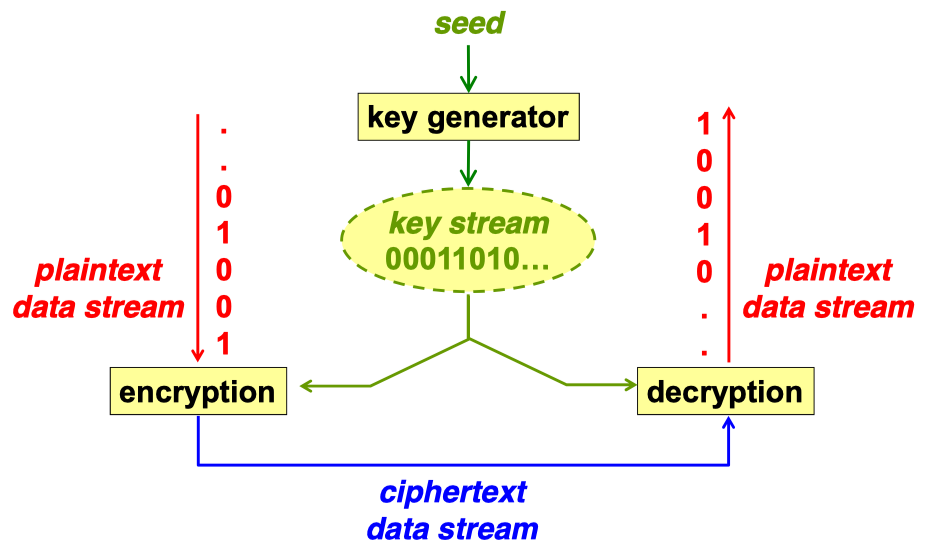
\includegraphics[width=\linewidth]{images/stream.png}
   \caption{Algorithms of type stream}
   \label{fig:stream}
\end{figure}
A lot of challenges were started for stream ciphers, some algorithms are:
\begin{itemize}
  \item HC-128, Salsa, SOSEMANUK
  \item Grain v1, MICKEY 2.0
  \item Salsa20 and ChaCha20
  \item Camellia
  \item SEED and ARIA
\end{itemize}

\paragraph{Problem of symmetric cryptography} one of the main problem of all this technique is that one key is required for each couple / group of user in order to guarantee privacy within groups. This means that, for a complete private communication between N parties, \textbf{$N*(N-1)/2$} keys are necessary, these require key exchange algorithms and generate a problem for large groups.\\
Another know problem is the \textbf{length of secret keys}, if:
\begin{itemize}
  \item The encryption algorithm was well designed
  \item the keys - N bit length - are kept secret
\end{itemize}
... then the only possible attack is the brute force (exhaustive) attack which requires a number of trials equal to:
\begin{center}
  $T = 2^{Nbit}$
\end{center}
This means that and increase of the computational power, reduce the strenght of the keys, that require a growning number over years. For this reason a challenges (AES) was promoted to develop another algorithm, the winner was \textbf{Rijndael}.

\subsection{Asymmetric Cryptography}
The Asymmetric Cryptography is based on 2 different keys generated in pairs, the two keys are different, one is called \textit{public} (\textbf{Kpub}) and the other \textit{private} (\textbf{Kpri}). If one key is used for encryption then the other one must be used for decryption, they have an inverse functionality. The computation load is high, due to this fact asymmetric encryption is used only for data streams and should not be used for data storage. The figure \ref{fig:asymmetric} show the process. The principals algorithms are:
\begin{itemize}
  \item Diffie-Hellman, RSA, DSA, El Gamal, etc...
\end{itemize}
\begin{figure}[H]
   \centering
   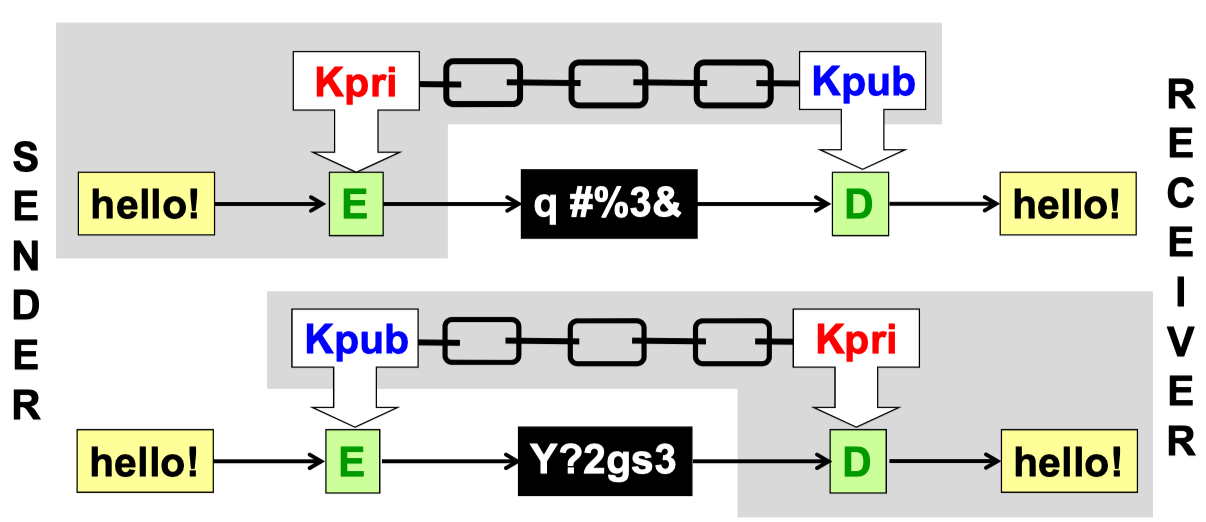
\includegraphics[width=\linewidth]{images/asymmetric.png}
   \caption{Asymmetric Cryptography with pairs of keys}
   \label{fig:asymmetric}
\end{figure}
Another possible application os this kind of cryptography is the \textbf{Digital Signature}, used to provide data authentication and integrity. Usually not all the data is encrypted but only its summary (\textbf{\textit{digest}}).\\
Another important feature is the possibility to make secret message for a particular receiver given only its public key.\\

\subsubsection{RSA}
This algoritmh is based on a public module:
\begin{center}
  \textbf{$N=P * Q$}
\end{center}
known to anybody P and Q are \textbf{\textit{prime number, large and secret}}. Another value, $PHI=(P-1)(Q-1)$, along a public exponent E such that arbitrarily $1<E<PHI$ and it is relative prime with respect to PHI.\\
From these element, a private exponent is computed:
\begin{center}
    $D=E^{-1}mod(PHI)$
\end{center}
from this last value the 2 keys can be computed:
\begin{itemize}
  \item public key = (N, E)
  \item private key = (N, D)
\end{itemize}
\textbf{After that computation P and Q must be deleted, discarded, killed!!!} Otherwise the process can be inverted.\\
An important note about RSA is that it can cipher/decipher only data whose value is less than the value of the module N, similar to a block algorithm but with a variable lenght. The final result is computed:
\begin{itemize}
  \item encrypt: $c = p^E mod(N)$
  \item decrypt: $c = p^E mod(N)$
\end{itemize}
For matematichal reasons the roles of the 2 exponents, E and D, are interchangeable:
\begin{center}
  $(x^D)^E mod(N) == (x^E)^D mod(N)$
\end{center}
The advantage of using modular arithmetic is that the inverse of a reminder of a module could be "any number", there are infinite possibilities. An example in figure \ref{fig:example_rsa}:
\begin{figure}[H]
   \centering
   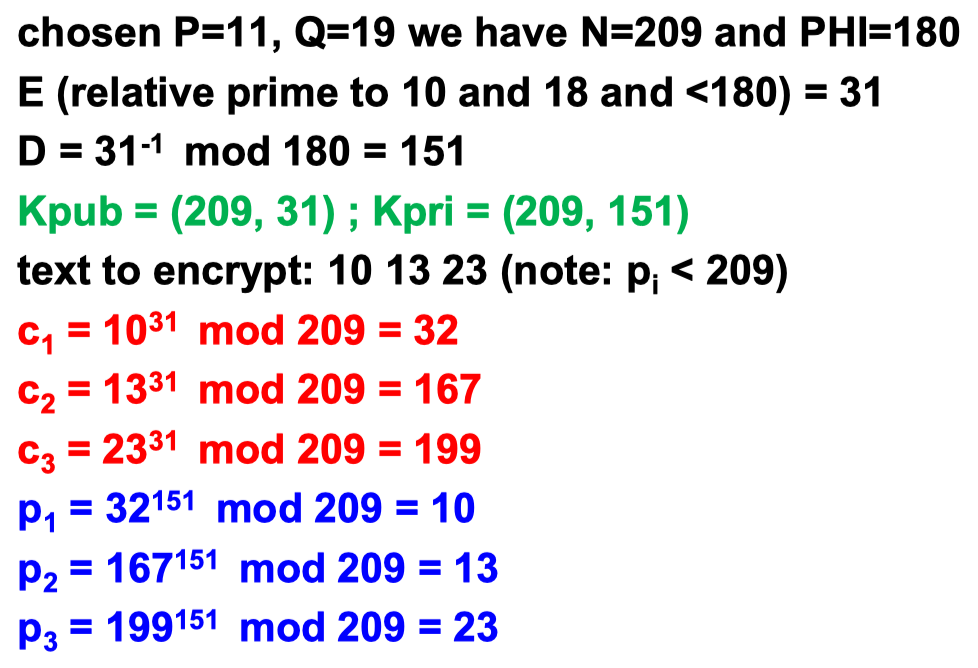
\includegraphics[width=\linewidth]{images/example_rsa.png}
   \caption{RSA an example}
   \label{fig:example_rsa}
\end{figure}
During years some optimizations were developed, like the one based on the CRT (Chinese Remainder Theorem) that makes the procedure 4x times faster.

\paragraph{Weaknesses} There are some know weaknesses:
\begin{itemize}
  \item Small encryption exponent
  \item Same keys for encryption and signing
  \item Acting as an oracle
\end{itemize}
Nowadays the lenght of the keys is important:
\begin{itemize}
  \item 512 bits keys $\sim$ Some weeks
  \item 1024 bits keys $\sim$ Some Months
  \item \textbf{2048 bits keys $\sim$ Several Years}
\end{itemize}

During Eurocrypt of 1999 a devices for decrypting RSA faster was annouced, it has never been presented, probably for interest reasons. For that, some governments, no longer want to use RSA solutions.\\

\subsubsection{Key Distribution}
The distribution is a fundamental step of asymmetric cryptography, the private key must kept SECRET, the ublic instead must be distributed as widely as possible. But how is possible to guarantee the binding between public key and person identity? There are 2 possible solutions:
\begin{itemize}
  \item Exchange of keys Out-Of-Band (e.g. keys party)
  \item Distribution by specific data structure (public key certificate)
\end{itemize}

Confidentiality without shared secrets is often used to send the secret key chosen for a symmetric algorithm, looking at figure \ref{fig:no_share}.
\begin{figure}[H]
   \centering
   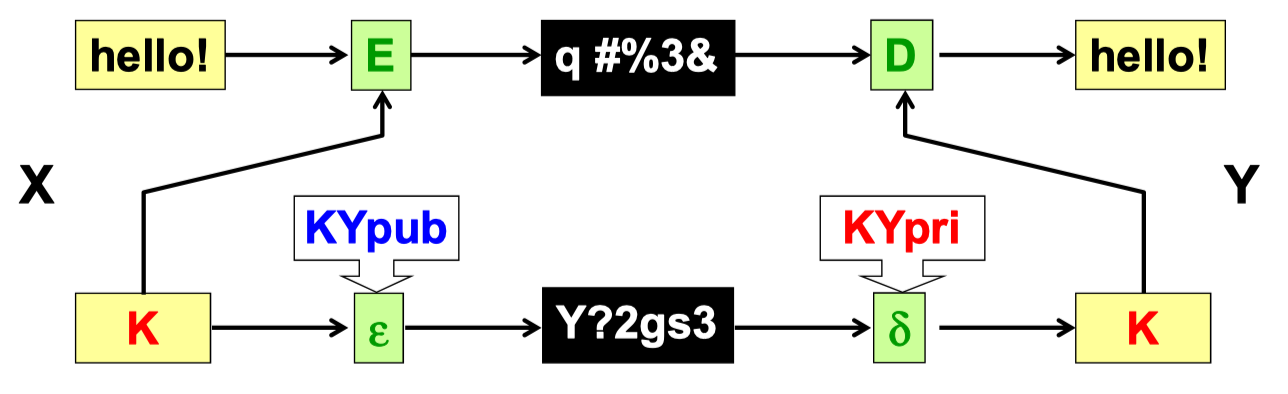
\includegraphics[width=\linewidth]{images/no_share.png}
   \caption{Confidentiality, no shared secret}
   \label{fig:no_share}
\end{figure}

\subsubsection{Diffie-Hellman}
Is the other well-know algorithm for asymmetric encryption. The idea behind the DH algorithm is good represented by figure \ref{fig:dh}.
\begin{figure}[H]
   \centering
   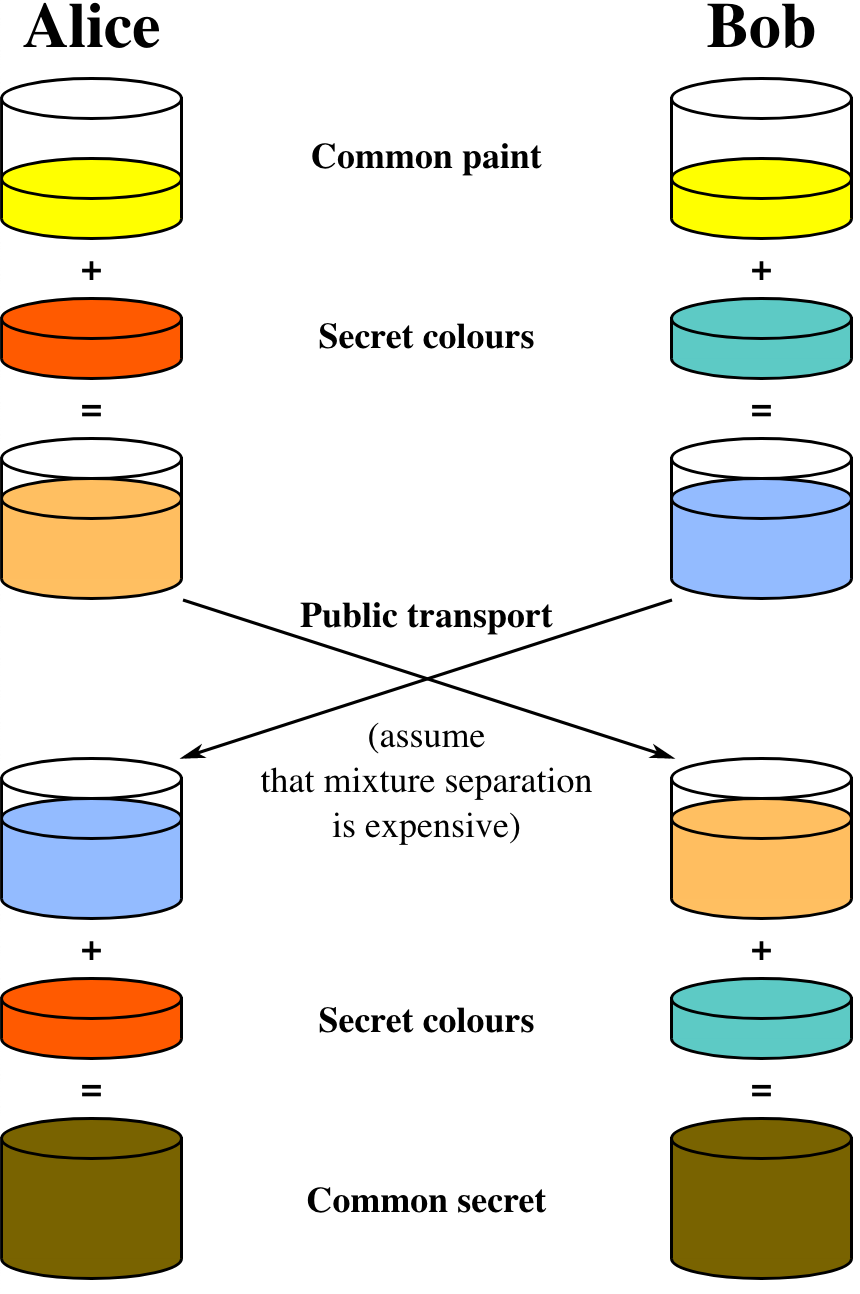
\includegraphics[width=\linewidth]{images/dh.png}
   \caption{Diffie-Hellman idea}
   \label{fig:dh}
\end{figure}
It was the first developed public-key algorithm, is frequently used to agree on a sceret key (\textit{key agreement}), it was patented but is now expired. One advantage is that is sniffing resistant. It can be exploited by a MITM attack by manipulating the data like in figure \ref{fig:dh_mitm}.
\begin{figure}[H]
   \centering
   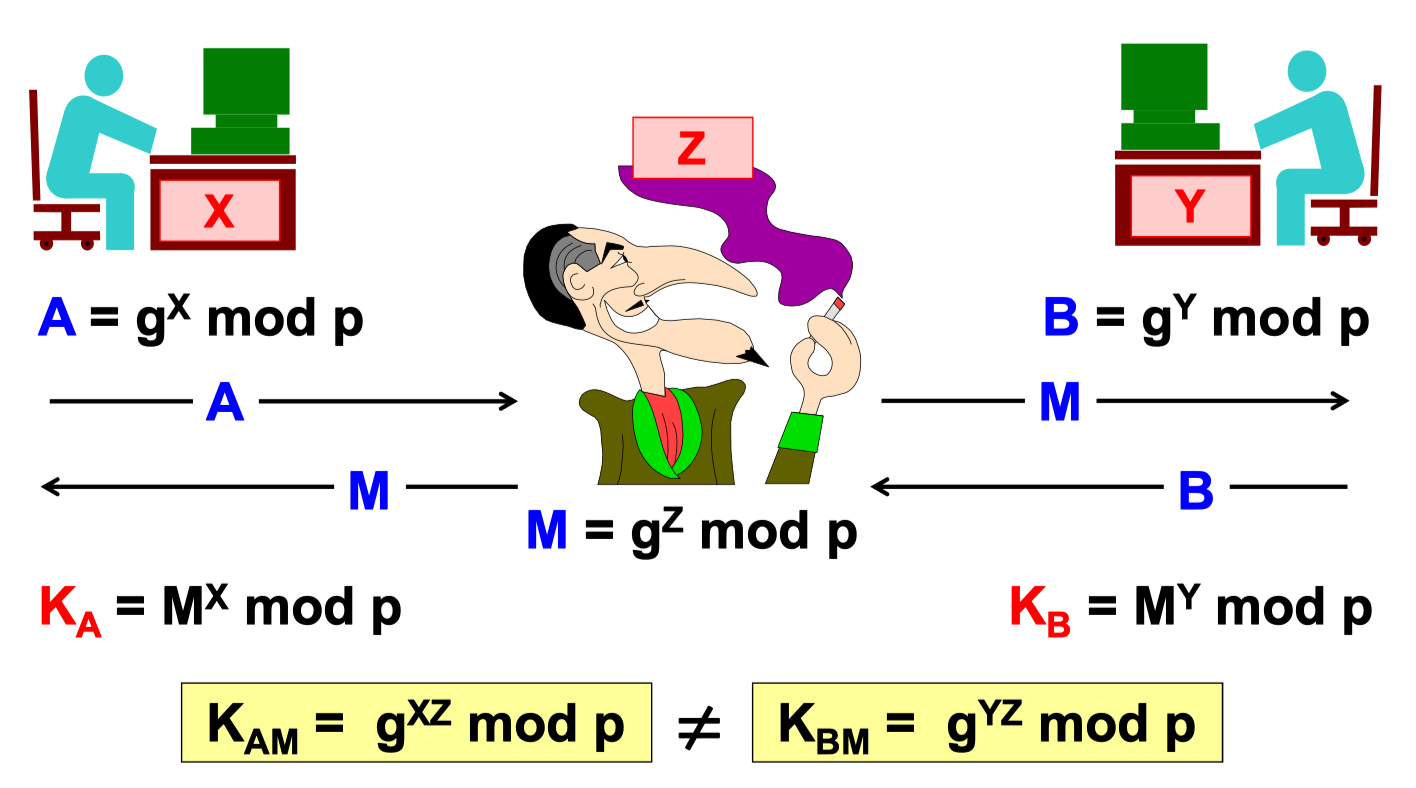
\includegraphics[width=\linewidth]{images/dh_mitm.png}
   \caption{Diffie-Hellman MITM}
   \label{fig:dh_mitm}
\end{figure}

The complexity of DH is a discrete logarithm, in any case also RSA, required the usage of quantum computer to be exploited in a reasonable amount of time.

\subsection{Elliptic Curve Cryptography}
This solution instead of using modular arithmetic, the operations are executed on the surface of a 2D (elliptic) curve. The problem of discrete logarithm on such a curve is more \textbf{more complex} than modular and allows \textbf{shorter keys} (about 1/10). A lot of algorithms has been rewritten, \textbf{EC}DSA or \textbf{EC}DH.\\

\paragraph{ECDH} the EC version of Diffie-Hellman is the same as before but with the math of an elliptic curve.\\
\begin{itemize}
  \item A and B select same elliptic curve and a point G of its
  \item A chose a random value x and computes: $X = x G$
  \item B chose a random value y and computes: $Y = y G$
  \item A and B exchange (publish) X and Y
  \item A computes $K = x Y$
  \item B computes $K' = y X$
\end{itemize}
but the final result will be that:
\begin{center}
  $K = K' = x y G$
\end{center}
There are also other algorithms like ECDSA:
\begin{itemize}
  \item Message digest computed with normal hash function (SHA-256)
  \item Signature = pair of scalars derived from the digest plus some operations on the curve
\end{itemize}
The ECIES instead:
\begin{itemize}
  \item Generates a symmetric encryption key (AES-128) with operations on the curve
  \item Gives to the receiver the information (based on his public key) needed to recompute the encryption key
\end{itemize}

\subsection{Integrity}
In most of the cases the real needes of the people around the world is not the secrecy of the data, but is its integrity. Intercepting a communication and change it, in an unpredictable way, could be worse than read it. For this reasons the digest come in.\\
The \textbf{digest} is a summary of something, the name is related to the \textit{reader digest} a magazine with the \textit{summary} of famous books.\\
The message digest is a fixed-length summary of the message to be protected (of any lenght). Is important for a digest to be of a fixed-size without depending upon the lenght of the data to be summarizzed. It must be:
\begin{itemize}
  \item \textbf{FIXED-SIZE}
  \item Fast to compute
  \item Impossible (or very difficult) to invert
  \item Difficult to create "collisions"
\end{itemize}
The digest is often used to avoid performing operations on the whole message, especially when the message is very large (slow pub-key crypto). The digest can be calculated in many ways, usually is calculated via \textbf{\textit{(Cryptographic)} Hash Function}.
The hashing algorithms are the faster in the world of cryptography, more than the symmetric ones and more than asymmetric, that are the slower.\\

The flow is simple (figure \ref{fig:digest}), the message M is splitted in N blocks $M_{1} ... M_{N}$, the blocks are then computed by a base function $f$. Each block generate and hash code:
\begin{center}
  $V_k = f(V_{k-1}, M_k)$
\end{center}
For the first block the $V_0 = IV$ (Initialization Vector), public and specified by the algorithm code. The digest is generated by the last computation of the function:
\begin{center}
  $hash = V_{N}$
\end{center}
\begin{figure}[H]
   \centering
   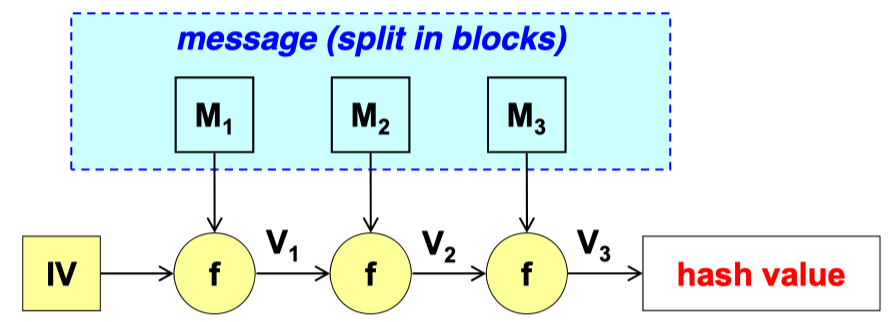
\includegraphics[width=\linewidth]{images/digest.png}
   \caption{Hashing flow}
   \label{fig:digest}
\end{figure}
The table show some advice about digest algorithms:
\begin{figure}[H]
   \centering
   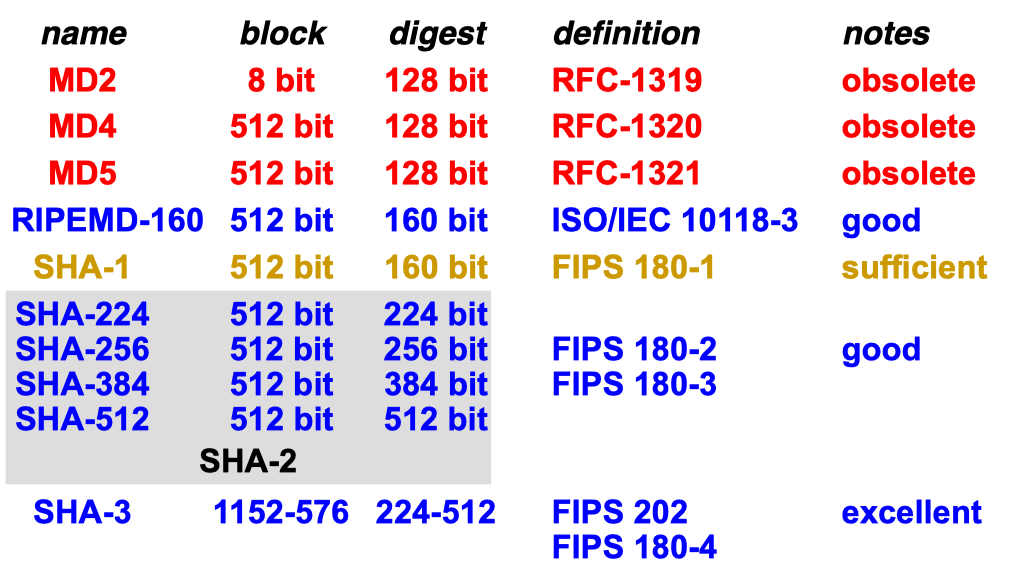
\includegraphics[width=\linewidth]{images/digest_alg.png}
   \caption{Digest Algorithms}
   \label{fig:digest_alg}
\end{figure}

The lenght of the digest is important, must be long enough to avoid \textbf{\textit{aliasing}
= Collisions}:
\begin{itemize}
  \item md1 = h(m1)
  \item md2 = h(m2)
  \item if (\textbf{m1 $\neq$ m2}) $\Rightarrow$ md1 $\neq$ md2
\end{itemize}
For an algorithm well designed the probability of aliasing is:
\begin{center}
  $P_A \propto 1/2^{Nbit}$
\end{center}
for this reasons digest function requires a good number of bits (birthday paradox).\\

The are some code used to guarantee the integrity of the messages: \textbf{MIC} \textit{(Message Integrity Code)}, to guarantee the authentication: \textbf{MAC} \textit{(Message Authentication Code)} and to avoid the replay attacks \textbf{MID} \textit{(Message IDentifier)}.

\subsection{Authentication}
The authentication is the process or action of verifying the identity of a user or process, or showing something to be true, genuine, or valid.
\subsubsection{Symmetric Cryptography}
Authentication can be performed in different ways. One possibility is the \textbf{auth by Symmetric Encryption}. This solution send also an encrypted copy of data:
\begin{itemize}
  \item (sender) M* = enc(K, M)
  \item (transmission) M $||$ M*
  \item (receiver) X = dec(K, M*)
  \item (verification) if (X == M) $\Rightarrow$ OK, else ALARM
\end{itemize}
Using this technique only who knows the (secret) key can compare the copy with the original. The disadvantage is that the performance are really poor, every operation must be executed 2 times, also the transmission.\\
Another similar technique is the \textbf{authentication by digest and symmetric encryption}, the adavantages are the data transmission is not doubled and only a digest is sent. The drawback is that two operations are required (digest + encryption).
\begin{itemize}
  \item (sender) H = enc(K, hash(M))
  \item (transmission) M $||$ H
  \item (receiver) X = dec(K, H)
  \item (verification) if (X == hash(M)) $\Rightarrow$ OK, else ALARM
\end{itemize}
Is also possible to enforce authentication by means of \textbf{keyed-digest}, in this solution the digest sended along with the data is calculated over data an a private key together.
\begin{itemize}
  \item (sender) d = digest(K, M)
  \item (transmission) M $||$ d
  \item (receiver) d* = dec(K, M)
  \item (verification) if (d == d*) $\Rightarrow$ OK, else ALARM
\end{itemize}
The solution require less overhead and only a single operation.
One of the most used solution is the \textbf{HMAC} where:
\begin{center}
  $hmac = H(K' \oplus opad || H(K' \oplus ipad || data))$
\end{center}
In case of size problem CBC-MAC can be used, it exploits a block-oriented symmetric encryption algorithm, in CBC mode with null IV, taking MAC as last encrypted block.
Both these solution are good, the only problem is the secret \textbf{shared} key, because the identity of the signer can't be distinguished, for the reasons is not good to be use in a commercial environment.\\
How is possible to combine both integrity and secrecy?
\begin{itemize}
  \item Secrecy = Symmetric Encryption with $K_{1}$
  \item Integrity = Keyed-digest (MAC) with $K_{2}$
\end{itemize}
Some possibilities are:
\begin{itemize}
  \item Auth\&Encr (eg. SSH)
  \begin{itemize}
    \item enc(p, $K_{1}$) $||$ mac(p, $K_{2}$)
    \item Need decrypt before check integrity
  \end{itemize}
  \item Auth-then-Encr (eg. TLS and SSL)
  \begin{itemize}
    \item enc(p $||$ mac(p, $K_{2}$), $K_{1}$)
  \end{itemize}
  \item Encr-then-Auth (eg. IPsec)
  \begin{itemize}
    \item enc(p, $K_{1}$) $||$ mac(enc(p, $K_{1}$), $K_{2}$)
  \end{itemize}
\end{itemize}
Improper combination of secure algorithms may leed to an insecure result!\\
The AE tecniques allows to achieve both privacy and authentication (and integrity):
\begin{itemize}
  \item One key
  \item One algorithm
  \item Better Speed
  \item Less error in combining
\end{itemize}
Are often used in applications, e.g. emails, networks, etc...\\
The RFC 5116 release define Interface and algorithms for authenticated encryption , for example the AEAD in figure \ref{fig:aead}.
\begin{figure}[H]
   \centering
   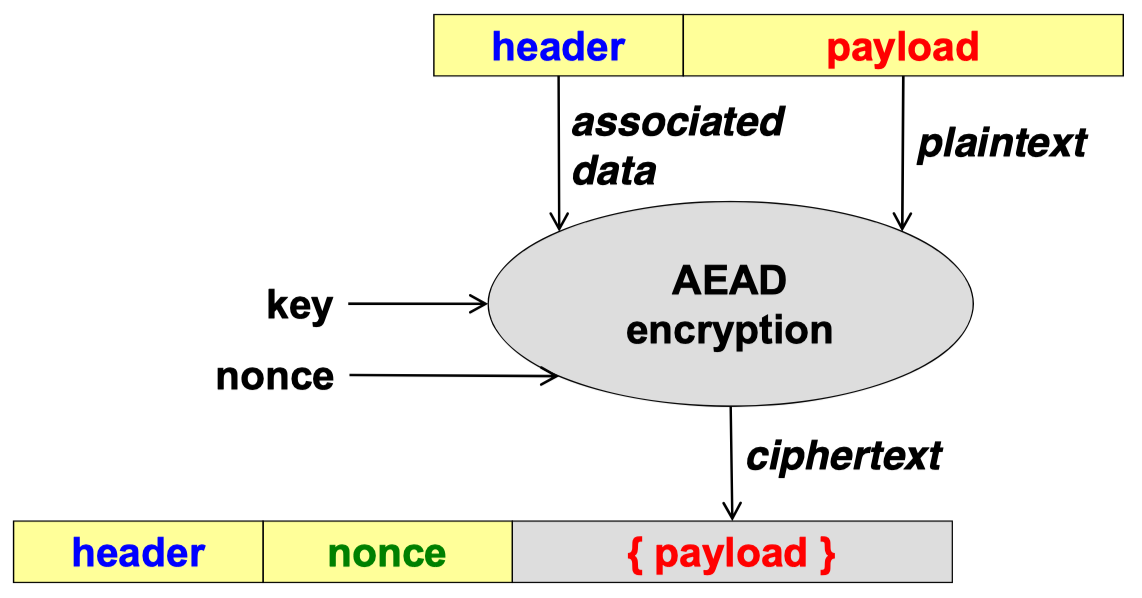
\includegraphics[width=\linewidth]{images/aead.png}
   \caption{Authenticated Encryption with Asociated Data (AEAD)}
   \label{fig:aead}
\end{figure}
The idea of AEAD is that comparing the two header, the one ciphered and the plain one, will guarantee the integrity.\\
The \textbf{IGE} (\textit{Infinite Garble Extension}) is a modde of application and is not too much used because is too simple to be exploited, the flow is in figure \ref{fig:ige}.
\begin{figure}[H]
   \centering
   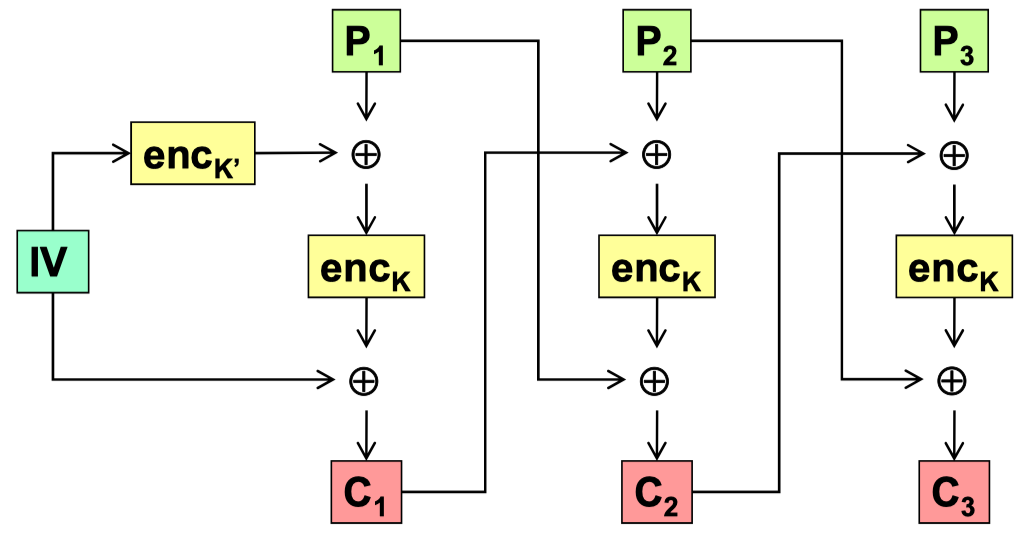
\includegraphics[width=\linewidth]{images/ige.png}
   \caption{IGE (Infinite Garble Extension)}
   \label{fig:ige}
\end{figure}
The AE standard are:
\begin{itemize}
  \item OCB 2.0
  \item AESKW (AE Key Wrap)
  \item CCM (CTR mode with CBC-MAC)
  \item EAX
  \item Encrypt-then-MAC
  \item GCM
\end{itemize}

\subsubsection{Asymmetric Cryptography}
Authentication can be also achieved by using \textbf{asymmetric} encryption. For example the \textbf{auth by digest and asymmetric crypto} is one of the first implementations:
\begin{itemize}
  \item (signer S) H = enc(S\_Kpri, hash(M))
  \item (transmission) M $||$ H
  \item (verifier V) X = dec(S\_Kpub, H)
  \item (verification) if(x == hash(M)) $\Rightarrow$ OK, else ALARM
\end{itemize}
those who knows the public key of the sender can compare the transmitted digest with the digest calculated on the received data. This is also know as \textbf{Digital Signature}! The figure show the behaviour.
\begin{figure}[H]
   \centering
   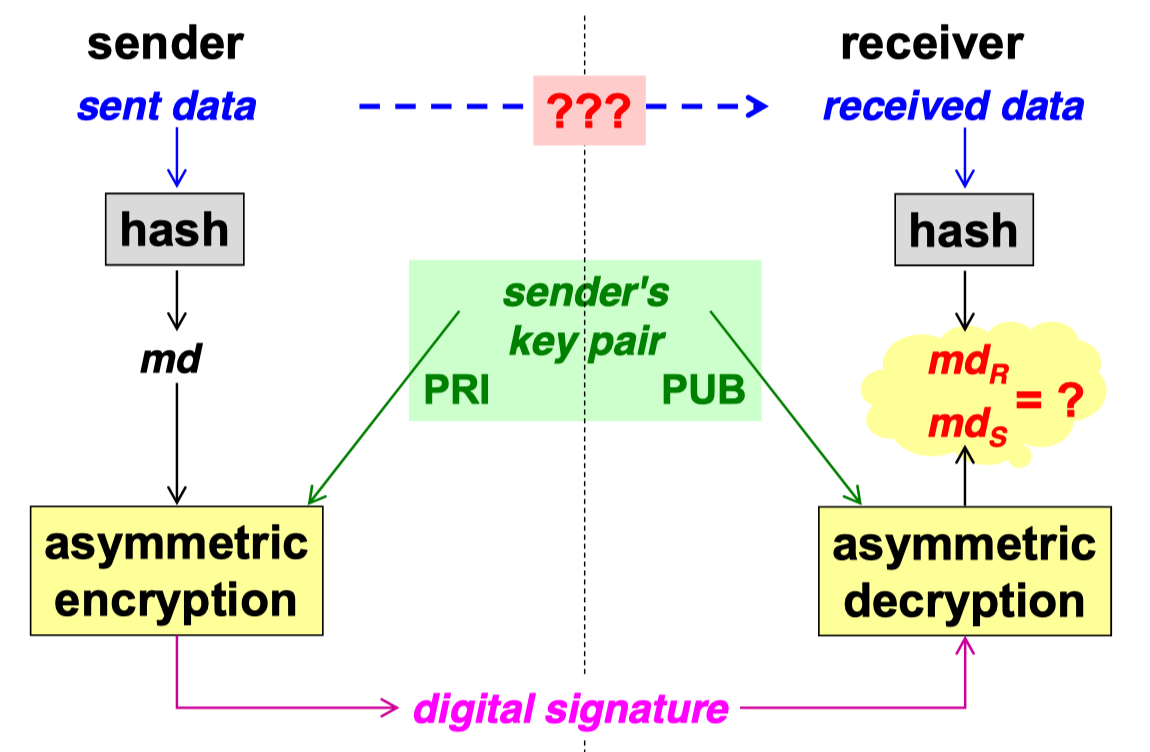
\includegraphics[width=\linewidth]{images/ds.png}
   \caption{Digital Signature}
   \label{fig:ds}
\end{figure}
DS can be achieved with RSA-based algorithms, they must be:
\begin{itemize}
  \item Resistant to collisions (even just to avoid generating accidentally the same signature)
  \item Difficult to invert
\end{itemize}

\subsubsection{Analysis}
The A-I by means of a shared secret:
\begin{itemize}
  \item Useful only for the receiver
  \item Cannot be used as a proof without disclosinng the secret key
  \item Not useful for non repudiation
\end{itemize}
Instead, by means of asymmetric encryption:
\begin{itemize}
  \item Being slow it is applied to the digest only
  \item Can be used as a formal proof
  \item Can be used for non repudiation
  \item = digital signature
\end{itemize}

The main advantage of a digital signature over an handwritten one is that it can guarantee both authentication and integrity because is tightly bound to the data.

\subsubsection{Public Key Certificate}
\textit{A data structure used to securely bind a public key to some attributes}, the idea is to bind a key to an identity, also other association are possible. The key will be digitally signed by the issuer: the \textbf{Certification Authority} for a limited amount of time. It can be revoked on request both by the user and the issuer.
Some of the most common formats for pub key certificates are:
\begin{itemize}
  \item X.509: ISO + IETF
  \item non X.509: PGP
  \item PKCS\#6: RSA
\end{itemize}
\paragraph{X.509} is oe of the most used certificate format, the structure il composed of:
\begin{itemize}
  \item Version
  \item Serial number
  \item Signature Algorithm
  \item Issuer
  \item Validity
  \item SUBJECT
  \item SUBJECT PubKeyInfo
  \item CA Digital Signature
\end{itemize}
An example in figure \ref{fig:x509}:
\begin{figure}[H]
   \centering
   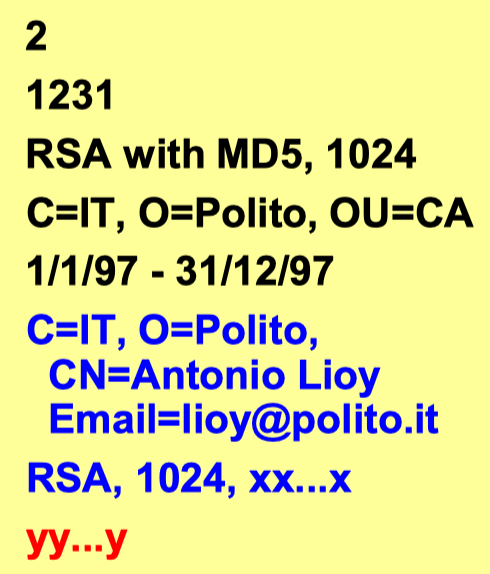
\includegraphics[width=\linewidth]{images/x509.png}
   \caption{X.509 Certificate Example}
   \label{fig:x509}
\end{figure}
The \textbf{PKI} (\textit{Public-Key Infrastructure}) is the Infrastructure, technical and administrative, put in place for the creation, distribution and revocation of public key certificates. Any certificate can be revoked before its expiration date:
\begin{itemize}
  \item By the owner
  \item By the creator
\end{itemize}
when a signature is verified, the receiver must (and is a responbilitity) check that the certificate was valid at signature time. There are 2 type or revocation mechanisms:
\begin{itemize}
  \item CRL (Certificate Revocation List):
  \begin{itemize}
    \item List of revoked certificates
    \item Signed by the CA or by delegated party
  \end{itemize}
  \item OCSP (On-line Certificate Status Protocol)
  \begin{itemize}
    \item Response containing information about certificates status
    \item Signed by the server
  \end{itemize}
\end{itemize}
How is made the verification of a signature? Look at figure \ref{fig:very_sign}.
\begin{figure}[H]
   \centering
   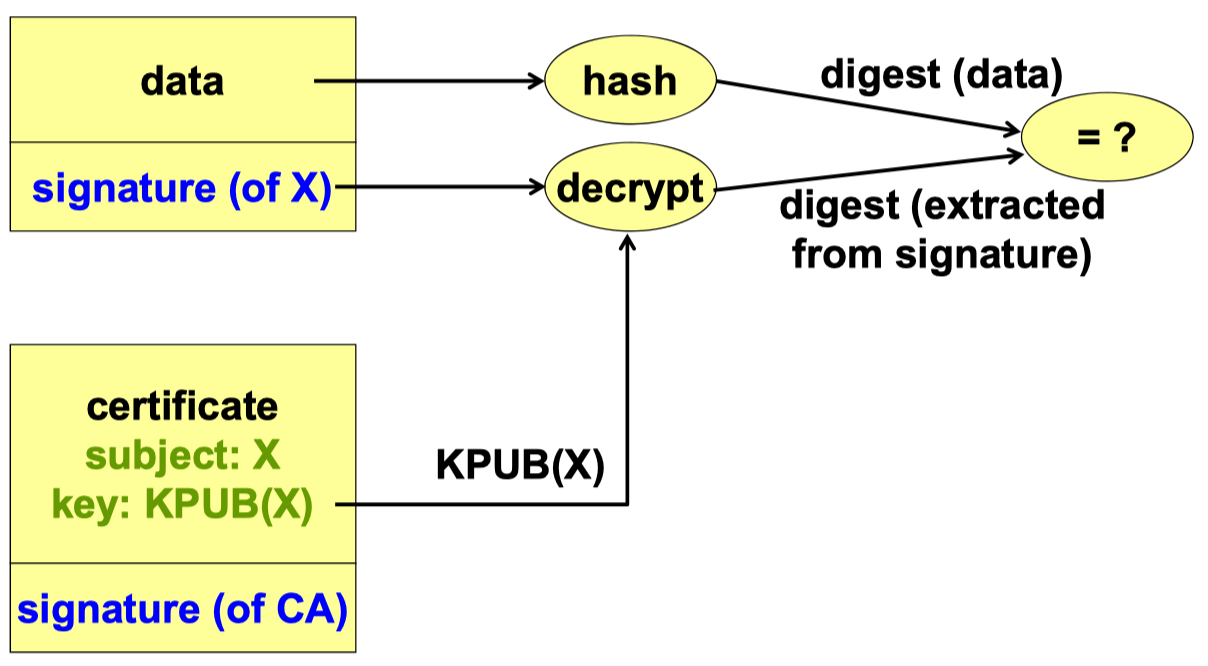
\includegraphics[width=\linewidth]{images/very_sign.png}
   \caption{Verification of signature/certificate}
   \label{fig:very_sign}
\end{figure}
A hierarchical Infrastructure is necessary to correctly verify the authenticity. At a certain point a TOP-LEVEL CA is needed, like "god". An example is showed in figure \ref{fig:ca_god}:
\begin{figure}[H]
   \centering
   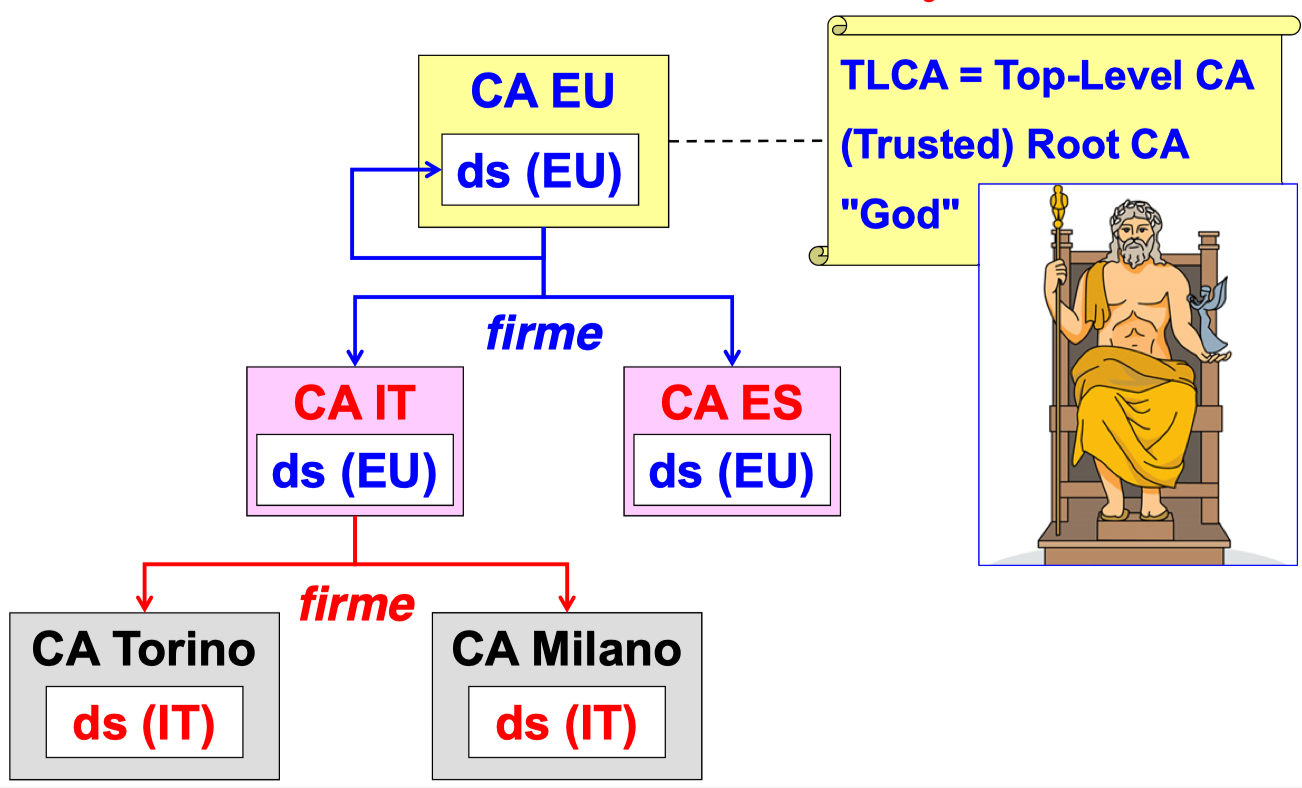
\includegraphics[width=\linewidth]{images/ca_god.png}
   \caption{Certification Hierarchy}
   \label{fig:ca_god}
\end{figure} % Ending basic_en.pdf

\newpage % Starting netsec_en.pdf
\section{Security of IP networks}
\subsection{Introduction}
Nowadays networks are become a fundamental basis of out life. Every devices is now connected or link the internet in some ways. The lead to a lot of security problem. Computers are faceing these issue from years, but refrigerators not. Is important to ensure a reliable and secure connections between the appliance and the internet world.

\subsection{Authentication}
The modern way to allow network access is to using an authentication protocol to an AAA server.
The most used protocol is the auth via PPP channels. \textbf{PPP} is a protocol to encapsulate network packets (LV3, e.g. IP) and charry them over a point-to-point link. I could be of different type:
\begin{itemize}
  \item Physical (RTC, ISDN)
  \item Virtual L2 (xDSL with PPPoE)
  \item Vistual L3 (L2TP over UDP/IP)
\end{itemize}
Activated in 3 sequential steps:
\begin{enumerate}
  \item LCP (Link Control Protocol)
  \item Authentication (optionall PAP, CHAP or EAP)
  \item L3 Encapsulation (IPCP, IP Control Protocol)
\end{enumerate}

The three possible protocols for authentications are:
\begin{itemize}
  \item \textbf{PAP} - Not more good!
  \begin{itemize}
    \item Password Auth Protocol
    \item Pwd send in clear
  \end{itemize}
  \item \textbf{CHAP}
  \begin{itemize}
    \item Challenge Handshake Auth Protocol
    \item Symmetric Challenge (based on user password)
  \end{itemize}
  \item \textbf{EAP} - Framework (USED)
  \begin{itemize}
    \item Extensible Auth Protocol
    \item External Techniques
  \end{itemize}
\end{itemize}
The EAP is a flexible L2 authentication framework, it use come predefined mechanis such as: MD5-challenge (similar to CHAP), OTP or Generic Token Card. Also other mechanisms may be added by the RFC standard, like the RADIUS support.\\
The authentication data are transported via its own encapsulation protocol (because L3 packets are not yet available), the main features are:
\begin{itemize}
  \item Indipendent of IP (Supports any link layers PPP, 802)
  \item Explicit ACK/NAK (no windowing)
  \begin{itemize}
    \item Assumes no reordering (PPP guarantees ordering, UDP or raw IP do not)
  \end{itemize}
  \item Rentransmission (3-5 max)
  \item No fragmentation
\end{itemize}
The link created by EAP is not assumed to be physically secure, EAP auth methods must provide security on their own. Some methods are:
\begin{itemize}
  \item EAP-TLS
  \item EAP-MD5
  \item EAP-TTLS
  \item EAP-SRP
  \item GSS\_API (ticket for Kerberos realm)
  \item AKA-SIM (Used for mobile SIM auth)
\end{itemize}
In figure \ref{fig:eap} the schema of EAP architecure:
\begin{figure}[H]
   \centering
   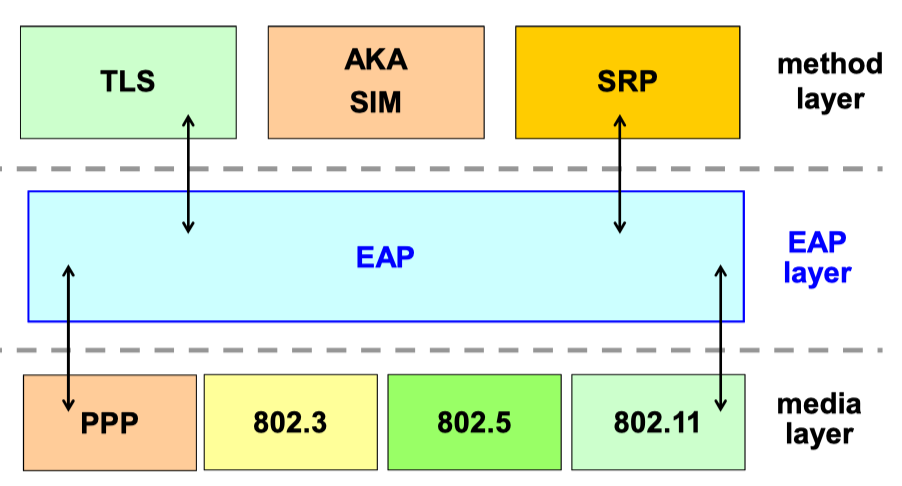
\includegraphics[width=\linewidth]{images/eap.png}
   \caption{EAP Architecture}
   \label{fig:eap}
\end{figure}
The request will be sended to a \textbf{NAS} (Network Access Server), the feature required by the NAS manufacturer are:
\begin{itemize}
  \item Authentication: \textit{Entity's identity is authenticated based on credentials}
  \item Authorization: \textit{Determining whether an entity is authorized to perform a given activity or access to resources}
  \item Accounting: \textit{Tracking network resource usage for audit support, capacity analysis or cost billing}
\end{itemize}
the Autentication Server performs these three functions talking with one or more NAS via one or more protocols.

\subsubsection{Authentication Protocols}
The most known are:
\begin{itemize}
  \item \textbf{RADIUS}: de-facto standard, proxy towards other AS.
  \item \textbf{DIAMETER}: evolution of RADIUS, roaming between different ISP, security.
  \item \textbf{TACACS+}: Better than RADIUS but proprietary solution of Cisco.
\end{itemize}

\paragraph{RADIUS} \textit{Remote Authentication Dial-In User Service} was developed in 1991 by Livingston technologies. It supports authentication, authorization and accounting to control network access, both on virtual and physical ports. It allow a centralized administration and accounting service, with a client-server schema between NAS and AS. It use port 1812 UDP for authentication and 1813 UDP for accounting.\\
One of the main feature is the ability to act like a proxy for other RADIUS db, an example is eudoram, that is the greatest RADIUS server in the world, and it's used by all the European University. In figure an example of work:
\begin{figure}[H]
   \centering
   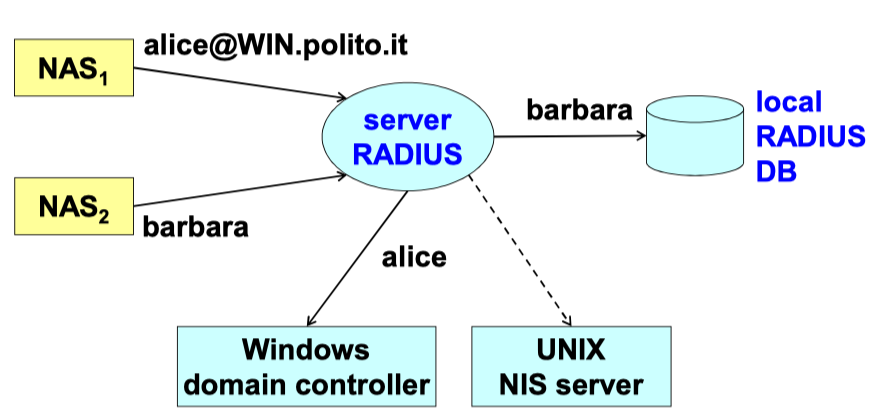
\includegraphics[width=\linewidth]{images/radius.png}
   \caption{RADIUS example}
   \label{fig:radius}
\end{figure}
Some security functions over attacks are implemented:
\begin{itemize}
  \item Sniffing NAS request
  \item Fake AS response
  \item Chaging AS response
  \item PWD enumeration
\end{itemize}
Packet integrity and authentication via keyed MD5:
\begin{center}
  $pwd \oplus MD5(key+authenticator)$
\end{center}
The user authentication via PAP, CHAP, token-card or EAP. The attributes are in TLV form, easily extensible without modification installed base. The types of the packet can be ACCESS-:
\begin{itemize}
  \item REQUEST: Contains access credentials
  \item REJECT: Access is denied
  \item CHALLENGE: Request additional info from the user
  \item ACCEPT: Access granted + network parameters given
\end{itemize}
Th RADIUS authentication has two pourpose, server reply authentication and no replay and masking the password. During the ACCESS-REQUEST step it is name Request Authenticator (16 byte randomly generated by the NAS), in the other steps is named Responde Authenticator and it is computed via keyed-digest:
\begin{center}
  $md5(code||ID||length||RequestAuth||atrtibutes||secret)$
\end{center}
The attributes of the RADIUS are:
\begin{itemize}
  \item type=1 (Username) - Network Access Identifier
  \item type=2 (User password)
  \item type=3 (Chap password)
  \item type=60 (CHAP-Challenge)
\end{itemize}
The NAI has been defined by the RFC-2468 and is made of:
\begin{center}
  $NAI=username[@realm]$
\end{center}
the user name is the one used in the PPP authentication phase. The figure \ref{fig:chap_radius} shown the flow of the protocol.
\begin{figure}[H]
   \centering
   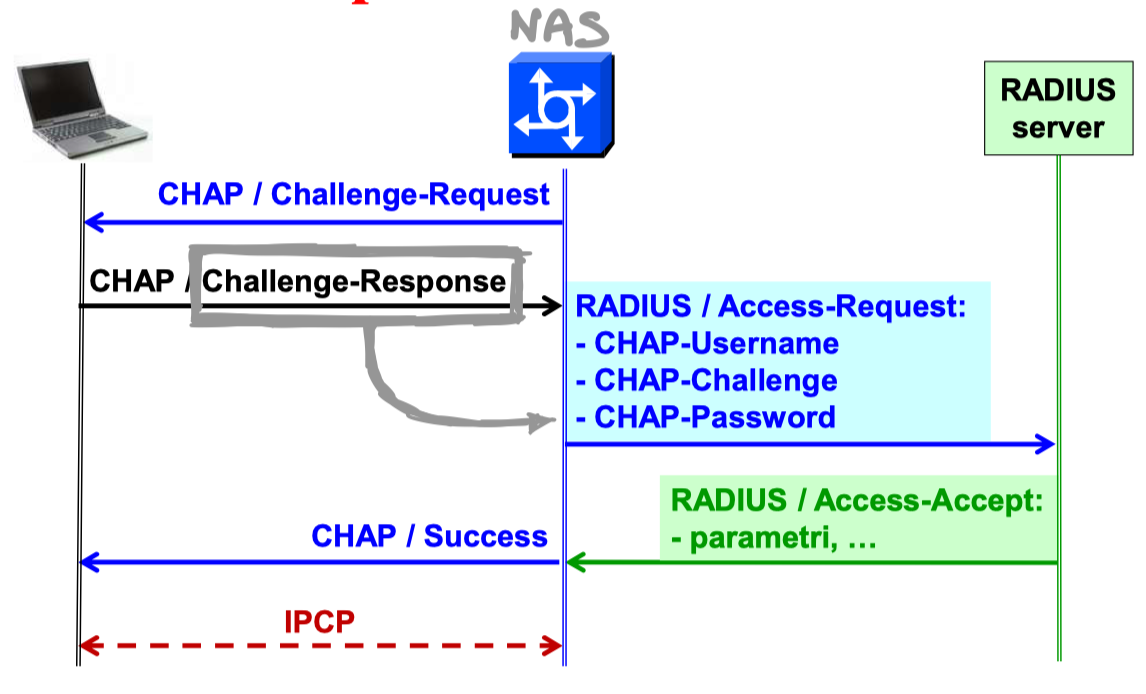
\includegraphics[width=\linewidth]{images/chap_radius.png}
   \caption{CHAP + RADIUS}
   \label{fig:chap_radius}
\end{figure}

\paragraph{DIAMETER} was developed like the RADIUS evolution (twice the radius), it has a special emphasis on roaming between ISPs. It guarantee protection via IPsec or TLS, both compulsory for the server side.

\paragraph{IEEE 802.1x} is a port-based Network Access Control: L2 architecture, usefull in a wired connection to block access, absolutely needed in wireless networks. The first implementations was born for Windows and Cisco wireless access-point. Is an authentication and key-management framework, it can derive keys for management, authentication, integrity and secrecy of packets, using standard algorithms for key derivation like TLS, SRP, etc... It can also provide other security services.\\
The main advantages for 802.1x is that it exploits the application level for the actual implementation of the security:
\begin{itemize}
  \item Direct dialogue between supplicant and AS (NIC-NAS "pass-trough device")
  \item No cange needed on NIC and NAS to implement new mechanisms
  \item Perfect integration in AAA
\end{itemize}
\begin{figure}[H]
   \centering
   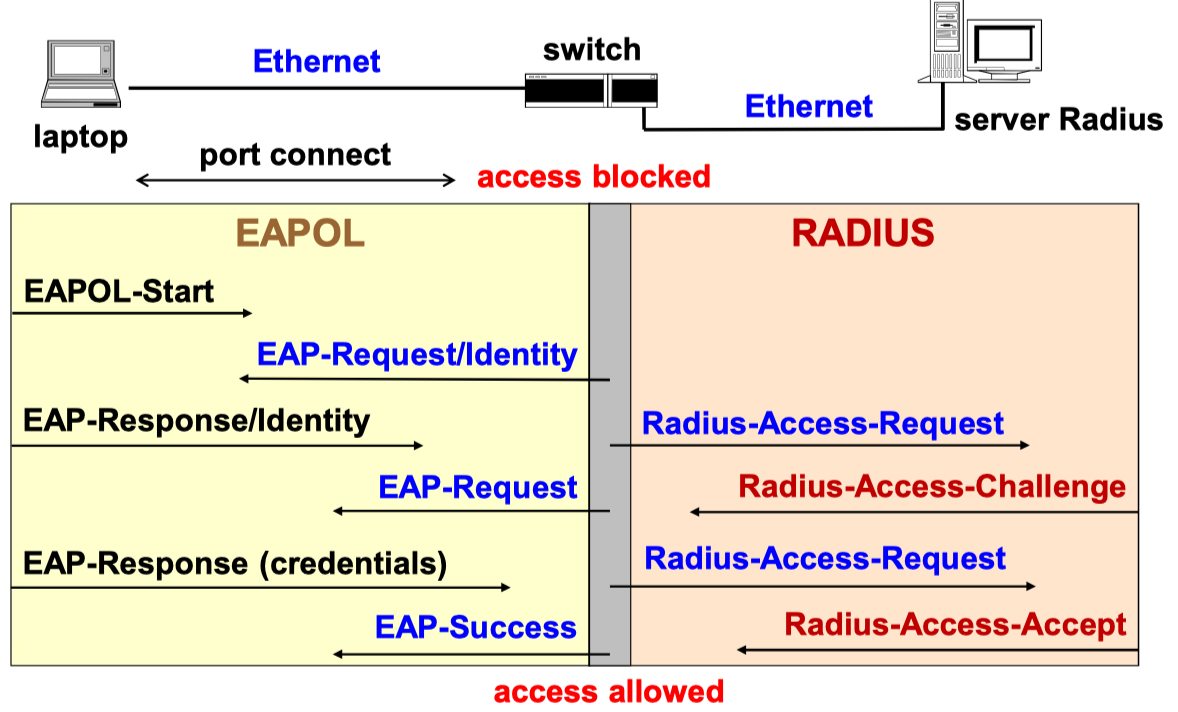
\includegraphics[width=\linewidth]{images/802-1x.png}
   \caption{802.1x Flow}
   \label{fig:802-1x}
\end{figure}

Which is the best level for apply security? The upper we go in the stack, the more specific are the security functions (e.g. Identify user, commands, data) and independent from the underlying network... But we leave more room for DoS attacks. The lower level we go in the stack, the more quickly we can expel the intruders, but we have also fewer data to make the decision (e.g. MAC, IP). The dest way is to put a little bit of security in every step of our stack. At low level, for faster expulsion, high level for more precise expulsion.

\subsection{DHCP}
DHCP is non-authentication protocol (really bad, trivial activation of shadow server). The main kind of attacks are:
\begin{itemize}
  \item DoS: Provides wrong configurations.
  \item MITM: Good configuration but /30 subnet, attacker like gateaway. With NAT also reply intercepted.
\end{itemize}
There are some solution to increase security but are not so much used, like DHCP snooping or HMAC-MD5 to authenticate messages (too complicated, required shared secret). In case a RADIUS server is available, is better to use it to gain network configurations.

\subsection{Security LV3 - VPN}
At LV3 security can be achived by two main solutions, securing all the networks, or by securing some paths.\\
What is a \textbf{VPN}? \textit{Virtual Private Network} is a technique hardware and/or software to create a private network while using a shared (or anyway untrusted) channels and transmission devices.
There are several techniques to create a VPN:
\begin{itemize}
  \item Private Addressing
  \item Protected Routing (IP Tunnel)
  \item Cryptography protection of the network packets (secure IP Tunnel)
\end{itemize}
The first, is not too much secure, the network to be part of the VPN use non-public addresses so that they are unreachable from other networks. This solution can be easily defeated if somebody discovers the addresses, it can sniff the packets during transmission and it has access to the communication devices.\\
The other solution, via Tunnel, use the router to encapsulate whole L3 packets as a payload inside another packet: IP-IP, IP-MPLS, other. THe router must perform access control to the VPN by ACL (Access Control List). This protection can be defeated by anybody that manages a router or can sniff packets during transmission. In figure \ref{fig:vpn_tunnel} a schema of the process:
\begin{figure}[H]
   \centering
   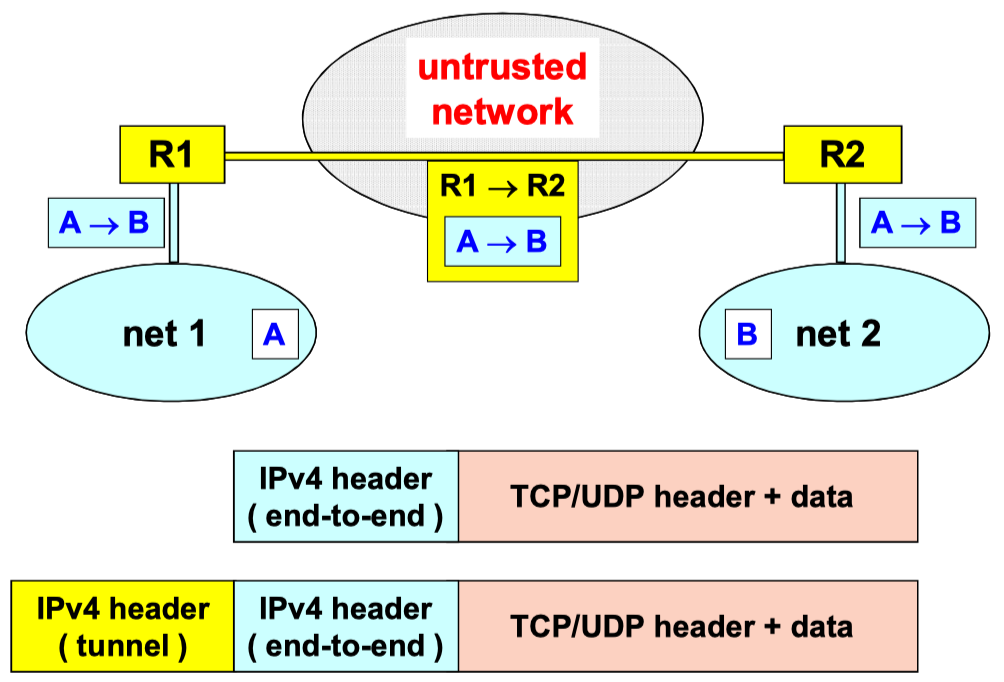
\includegraphics[width=\linewidth]{images/vpn_tunnel.png}
   \caption{VPN via IP Tunnel}
   \label{fig:vpn_tunnel}
\end{figure}
If packet has size equal to the MTU, then encapsulation will only possible with fragmentation, this means performance loss, that can't be grater than 50\%.\\
The best solution is the VPN via secure IP tunnel, before the encapsulation, the packets are protected with:
\begin{itemize}
  \item MAC (integrity + authentication)
  \item Encryption (confidentiality)
  \item Numbering (to avoid replay)
\end{itemize}
If the cryptographic algorithms are strong, then the only possible attack is to stop the communications. This solution is a.k.a as S-VPN (Secure VPN), figure \ref{fig:svpn}.
\begin{figure}[H]
   \centering
   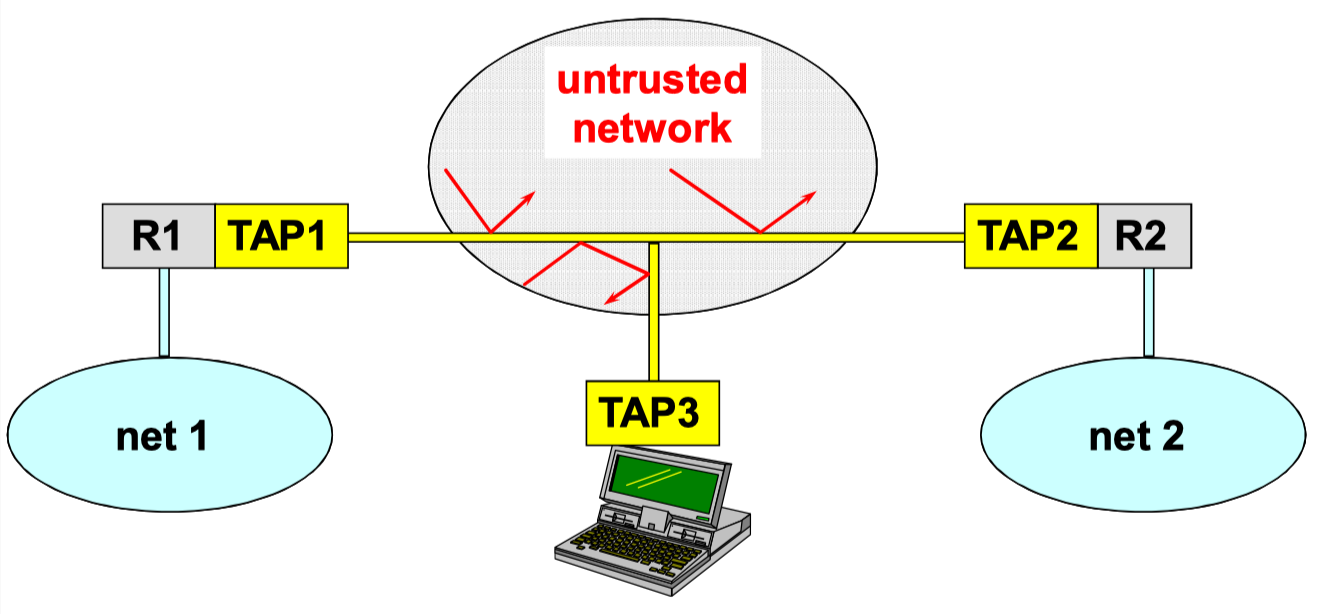
\includegraphics[width=\linewidth]{images/svpn.png}
   \caption{Secure VPN schema}
   \label{fig:svpn}
\end{figure}

\subsubsection{IPsec}
One of the most used VPN solution is \textbf{IPsec}, defined by IETF, is an architecture for L3 security in IPv4/IPv6, to create S-VPN over untrusted networks, or to create end-to-end secure packet flows. It defines to specific packet types:
\begin{itemize}
  \item \textbf{AH} (\textit{Authentication Header}): Integrity, Authentication, no replay
  \item \textbf{ESP} (\textit{Encapsulating Security Payload}): Confidentiality
\end{itemize}
It make use of IKE for keys exchange.\\
The \textbf{Security Association} (SA) is an unidirectional logic connection between two IPsec systems, two SA are needed to get complete protection of a bidirectional packet flows. Each SA is indipendent and it is associated with different security services, they can be also the same.\\
IPsec make use of some sort of DB for managing connections:
\begin{itemize}
  \item SAD (SA Database): Not a real DB, is the list of active SA and their characteristics
  \item SPD (Security Policy Database): List of security policy to apply to the different packet flows, configured a-priori or by an automatic system.
\end{itemize}
The \textbf{transport mode} of IPsec is used for end-to-end security, that is used by hosts, not gateways. The advantage is that is computationally light, the cons is that there isn't protection for the header variable fields. The \textbf{tunnel mode} instead, is used to create a VPN by gateways, the advantages are the protection of header variable, the problem is that is computationally heavy.\\
The AH, that ensure data integrity and sender authentication, the first version was supporting keyed-MD5 and optionally of keyed-SHA-1, now in ensure also (partial) protection from replay attack and it use HMAC-MD5-96 and HMAC-SHA-1-96. Figure \ref{fig:ipssec_flow} show the flow of the architecture.
\begin{figure}[H]
   \centering
   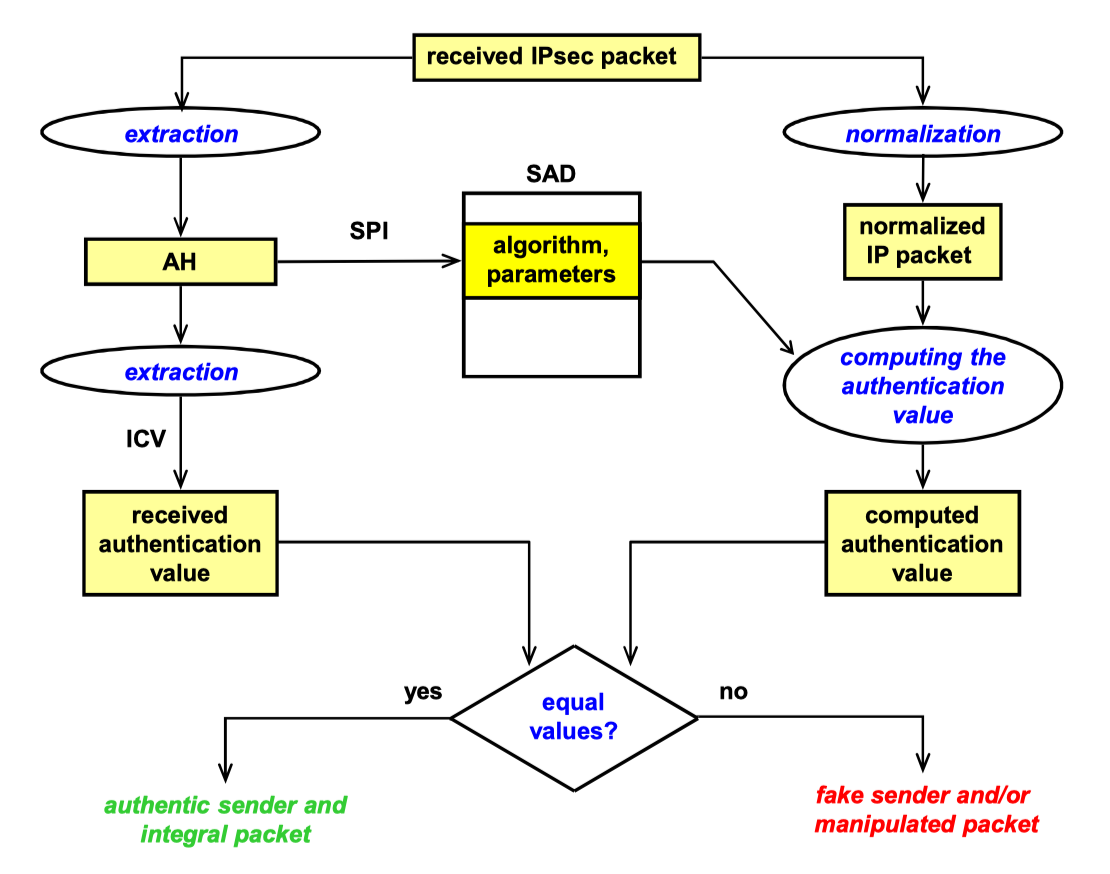
\includegraphics[width=\linewidth]{images/ipssec_flow.png}
   \caption{IPsec flows}
   \label{fig:ipssec_flow}
\end{figure}
The normalization of AH it reset the TTL and the Hop Limit Field. If the packet contains a ROuting Header, then:
\begin{itemize}
  \item Set the destination field to the address of the final destination
  \item Set the content of the routing header to the value that it will have at destination
  \item Set the Address Index field at the value that it will have at destination
\end{itemize}

\paragraph{ESP} (\textit{Encapsulating Security Payload}) is a solution to encapsulating IP packets. With the latest version is possible to provide confidentiality and authentication. Using it in trasport mode have some conseguence:
\begin{itemize}
  \item {+} Payload is hidden (including info needed for QoS, filtering or intrusion detection)
  \item {-} The header remains in clear
\end{itemize}
Using the tunnel mode something is changing:
\begin{itemize}
  \item {+} Hides both payload and (original) header
  \item {-} Larger packet size
\end{itemize}
The last implementation use the ESP-DES-CBC format.
\begin{figure}[h!]
  \centering
  \begin{minipage}{.48\textwidth}
    \centering
    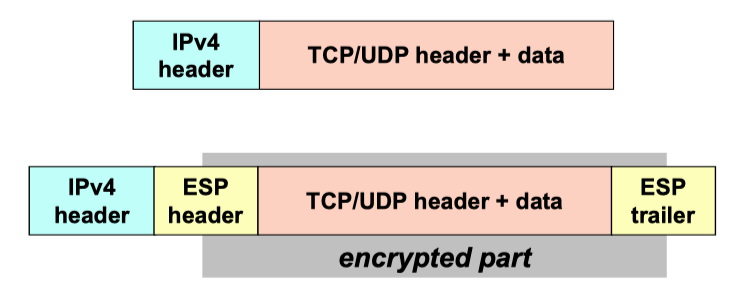
\includegraphics[width=\linewidth]{images/esp-transport.png}
    \caption{ESP: transport mode}
    \label{fig:esp-transport}
  \end{minipage}\hfill
  \begin{minipage}{.48\textwidth}
    \centering
    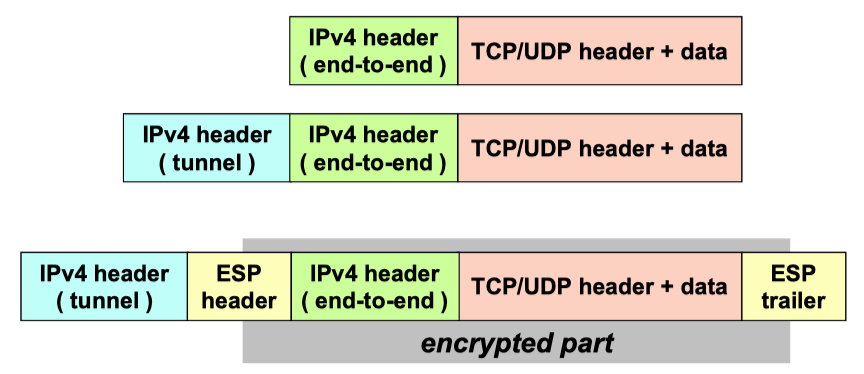
\includegraphics[width=\linewidth]{images/esp-tunnel.png}
    \caption{ESP: tunnel mode}
    \label{fig:esp-tunnel}
  \end{minipage}\hfill
\end{figure}

The IPsec implementation details are:
\begin{itemize}
  \item VPN-A: ESP/3DES-CBC/HMAC-SHA1
  \item VPN-B: ESP/AES-128-CBC/AES-XCBC-MAC-96
\end{itemize}
The NULL algorithms for ESP:
\begin{itemize}
  \item For authentication or privacy (not simultaneosly)
  \item Protection vs. performcae trade-off
\end{itemize}
Sequence Number:
\begin{itemize}
  \item Partial protection from replay
  \item Minimum window of 32 packets (64 suggested)
\end{itemize}
The real \textbf{replay protection} follow a sequence of actions:
\begin{enumerate}
  \item After SA is established, sender initilizes sequence number to 0
  \item For each packet the Seq.Numb is incrementend
  \item At the reach of the maximum sequence number, the new SA should be negotatiated
\end{enumerate}

The IPsec v3 use: AH is optional and ESP is mandatory, support for single multicast source, uses extended sequence number (64 bits), support AEAD and add some clarifications about SA and SPI (for faster lookup).
Multiple combinations of VPN can be exploited together in order to use of the different benefits between the different modes:
\begin{itemize}
  \item trasport-mode between to hosts
  \item tunnel-mode between to gateways
  \item 1st and 2nd together
  \item Host and gateways with tunnel mode
\end{itemize}

\paragraph{Key management} is one of the most important component of IPsec, is in charge of provides, to both parties, the symmetric keys used for packet authentication and/or encryption. The distribution can be achived in two ways:
\begin{itemize}
  \item OOB
  \item Automatic in-band
\end{itemize}
The protocol used by IPsec is the \textbf{ISAKMP} (\textit{Internet Security Association and Key Management Protocol}) it negotiate, set-up, modify and delete SA, the exchange is not fixed, the one used is OAKLEY.
The whole phase is managed by \textbf{IKE}, \textit{Internet Key Exchange}, it create SA to protect the ISAKMP exchange, this created SA is used to protect the negotiation of the SA needed by IPsec traffic, the same SA can be used several times to negotiate other IPsec SA.\\
The IKE flow is divided in two phases:
\begin{enumerate}
  \item Negotiation of a bidirectional ISAKMP SA: \textit{main or aggressive mode}
  \item Negotiation of the IPsec SA: \textit{quick mode}
\end{enumerate}
The different modes of operation are:
\begin{itemize}
  \item Main mode: 6 msg, protect parties identities
  \item Aggressive mode: 3 msg
  \item Quick mode: 3 msg, negotiation only of the IPsec SA
  \item (new) Group mode: 2 msg, already used for update SA parameters
\end{itemize}
The IKE process allows different authentication methods:
\begin{itemize}
  \item Digital Signature: non-repudiation of the IKE Negotiation
  \item Public Key Encryption: identity protection in the aggressive mode
  \item Revised Public Key Encryption: less expensive, only 2 public-key operations
  \item Pre-shared Key: party ID may only be its IP address
\end{itemize}
System requirement for IPsec appliance:
\begin{itemize}
  \item Router: Powerful CPU or Crypto AES-NI accelerator
  \item Firewall: Powerful CPU
  \item VPN Concentrator: (special-pourpose appliance terminator of IPsec tunnel)
\end{itemize}
Of course the IPsec tunnel encapsulation require a reduce of the throughput due to 2 main reasons:
\begin{itemize}
  \item Larger Packet Size: AH (+24 bytes), ESP-DES-CBC (>= 32 bytes)
  \item Larger number of packets: SA activation and update
\end{itemize}
Usually the decrease is not too much important, with a proper hardware, there are some exception like in Point-To-Point link that used L2 compression that now becomes useless or counterproductive when applied to ESP packets.

\subsubsection{IP insecurity}
The intrinsic insecurity of IP protocol drive insecurity to all the services transported by it, the main problem are the not authentication of addresses and the unprotected packets (integrity, authm confidentiality and replay).\\
\paragraph{ICMP} is the \textit{Internet Control and Management Protocol} the is vital for the network management, the main problem is that is used for many attacks because it has no authentication. Some example of attacks are:
\begin{itemize}
  \item Smurfing: Using broadcast addresses to lot of replay to a single host
  \item Fraggle: Similar to smurfing but with UDP packets
  \item ARP Poisoning
  \item TCP SYN Flooding: Multiple open connection TCP
\end{itemize}

\subsubsection{DNS}
The goal of the DNS is to translate from name to IP and from IP to name. Is a again a vital service, the query are performed over UDP@53, is not secured at all.\\
One of the main attacks performed exploiting DNS leak is the shadows server by sniffing to intercept the queries and spoofing to generate a fake answers. Other possible attacks are the DNS cache poisoning.\\
For a lot of reasons the \textbf{DNSsec} is needed to avoid attacks like the Kaminsky one (figure \ref{fig:kaminsky}), is now available from some public like Cloudflare DNS.
\begin{figure}[H]
   \centering
   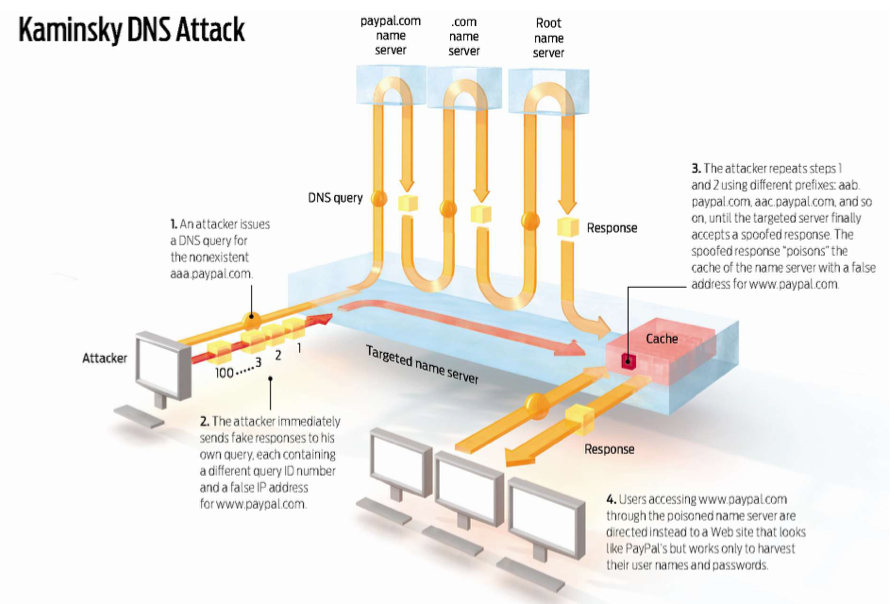
\includegraphics[width=\linewidth]{images/kaminsky.png}
   \caption{Kaminsky Attack}
   \label{fig:kaminsky}
\end{figure}
This new solution peform: Digital Signature of DNS records. It must face over some issues like not signed DNS response, no root CA, bigger record size and scarse experimental results.

\paragraph{Routing security} another low critical appliance are the router, normally they have low security management for accessing like telnet or SNMP, there is also low security in the exchange of routing tables.
% Ending NETWORK Security

\section{X.509}
The third version of X.509 was developed in June 1996, the goal is to groups together in a unique document the modifications required to extend the definition of certificate and CRL. Two types of fundamental extensions are available:
\begin{itemize}
  \item \textbf{Public}: That is defined by the standard and consequently made public to anybody
  \item \textbf{Private}: Unique for a centain user community
\end{itemize}
X.509 was useless before the idea of the extensions. The extensions can be defined critical and non critical:
\begin{itemize}
  \item In the verification process the certificates that contain an unrecognized critical extension MUST be rejected
  \item A non critical extension MAY be ignored if it is unrecognized
\end{itemize}
The different processing is entirely the responsibility of the party that performs the verification: the \textbf{Relying Party (RP)}.\\
The public extension classes defined by the v3 of X.509 include:
\begin{itemize}
  \item Key and Policy information: Author, subject, key usage, etc...
  \item Certificate subject and certificate issuer attributes
  \item Certificate path constraints: Basic, name and policy
  \item CRL distribution points
\end{itemize}
The \textbf{key usage} identifies the application domain for which the public key can be used (nonRepudiation, keyEnchipherment, dataEncipherment, keyAgreement, digital signature, cRLSign). It can be critical or not critical, if critical it can be used only for the scopes for which the corresponding option is defined.\\
The \textbf{Certificate Subject and Certificate Issuer Attributes} can have:
\begin{itemize}
  \item Subject Alternative Name (SAN): Different formalisms to identify the owner (Mail, IP, URL)
  \item Issuer Alternative Name
  \item Subject Directory Attributes
\end{itemize}
The Basic constraints is used to indicates if the subject of the certificate can act as a CA. If true, also the depth of the certification tree can be defined. It can be critical or non critical. The name constraint field is used only by CA, it define the space of names that can be ceritified by the CA and the possibility of subTree. The last possibilities, the CRL distribution point, identifies the distribution point of the CRL to be used in validating a certificate, it can be a directory entry, mail or URL and it can be critical or not.\\
The \textbf{Private Extensions} that is extensions common to a certain user community.

\subsection{CRL}
Is the certificate revocation list, they are issued periodically and maintained by the certificate issuers. Of course they are digitally signed:
\begin{itemize}
  \item By the CA that issued the certificates
  \item By a revocation authority delegated
\end{itemize}
A set of extensions have be developed for the CRLv2, the \textbf{crlEntryExtensions} and the \textbf{crlExtensions}. The timeline of a revocation is shown in the following figure:
\begin{figure}[H]
   \centering
   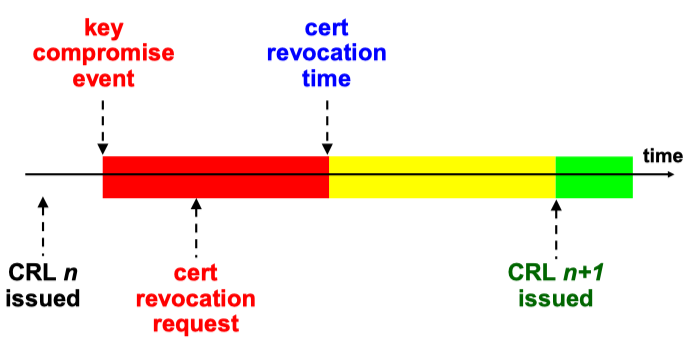
\includegraphics[width=\linewidth]{images/revoc_timeline.png}
   \caption{Revocation Timeline}
   \label{fig:revoc_timeline}
\end{figure}
The timeline is divided in three parts:
\begin{itemize}
  \item RED: Still valid certificate (Revocation requested)
  \item YELLOW: Cert still valid for who not already informed (dangerous)
  \item GREEN: Safe zone
\end{itemize}
When a key is issued is also important to verify the revocation time policy, they can varying from minutes to days. A solution to improve the efficency of this protocol is to use OCSP.\\
The \textbf{OCSP} \textit{Online Certificate Status Protocol} is a standard to verify online if a certificate is valid: Good, revoked or unknown. The response is signed by the server. The OCSP server certificate cannot be verified with OCSP itself.\\
The response of the OCSP server can be precomputed, this reduce the load over the server, but makes possible replay attacks. Is also possible to obtain information not from CRL. The responder can be of 2 types:
\begin{itemize}
  \item \textbf{Trusted}: Response signed with a pair key;cert independent of the CA for which it is responding. (Company responder or TTP paid by users)
  \item \textbf{Delegated}: The OCSP server signs the responses with a pair which is different based on the CA for which it is responding. (Paid by CA)
\end{itemize}

\subsection{Time stamping}
Is a really important feature. Is a proof of creation of data before a ceratin point in time, the requested is managed by a Time-Stamping Authority. The flow is the following:
\begin{figure}[H]
   \centering
   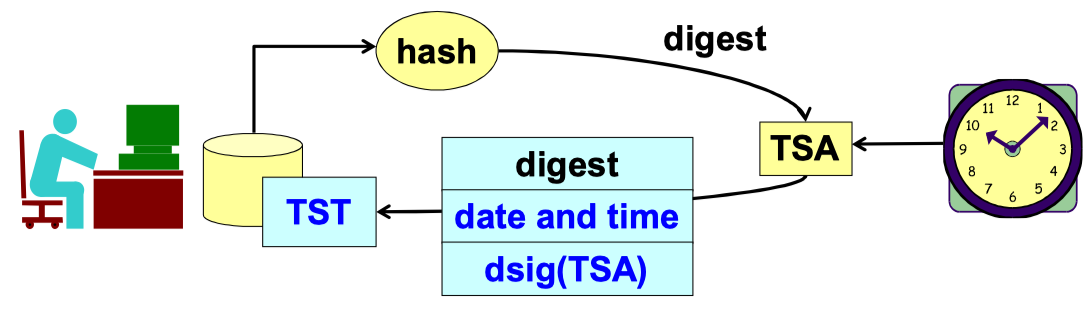
\includegraphics[width=\linewidth]{images/tpf.png}
   \caption{Time-Stamping procedure}
   \label{fig:tpf}
\end{figure}

\subsection{PSE: Personal Security Environment}
There are several types of solution in order to keep secure our data, from private key to certificates of the trusted root CAs. The PSE can be:
\begin{itemize}
  \item \textbf{Software}: Encrypted file of private key
  \item \textbf{Hardware}: Passive (Similar to SW) or Active (Protected keys + Crypto Operations)
\end{itemize}
An example of HPSE are the cryptographic smart-card, they are chip cards with memory and/or autonomous cryptographic capacity (DES or RSA and ECDSA). They are based on a small memory (EEPROM): 4-32 KByte. The basic idea is to not give the key to sign, but to get what must be signed.
The \textbf{HSM} (\textit{Hardware Security Module}) is a cryptographic accelerator for servers, securely store private key and have autonomous encryption capabilities.\\

\subsection{CMS}
The \textit{(Cryptographic Message Syntax)} is the evolution of the PKCS\#7 that is a RSA standard for secure envelope. It allows data authentication, integrity and/or privacy, with both symmetric and asymmetric algorithms. It supports mutiple signatures (hierarchical or parallel) on a signle object and can include the certs to verify the signature. The CMS can use several algorithms:
\begin{itemize}
  \item Digest: MD5, SHA-1
  \item Signature: RSA, DSA
  \item Key management:
  \begin{itemize}
    \item Agreement: DH
    \item Transport: RSA
    \item Symmetric Wrapping: 3DES, RC2
    \item Derivation: PBKDF2
  \end{itemize}
  \item Content Encryption: 3DES-CBC, RC2-CBC
  \item MAC: HMAC-SHA1
\end{itemize}
The structure of CMS is made of a contentInfo that contains the pieces: contentType and the content.
The contentType can be:
\begin{itemize}
  \item Data
  \item signedData (fig.\ref{fig:signedData})
  \item envelopedData (fig.\ref{fig:envelopedData})
  \item authenticatedData
  \item digestedData
  \item encryptedData
\end{itemize}
\begin{figure}[H]
   \centering
   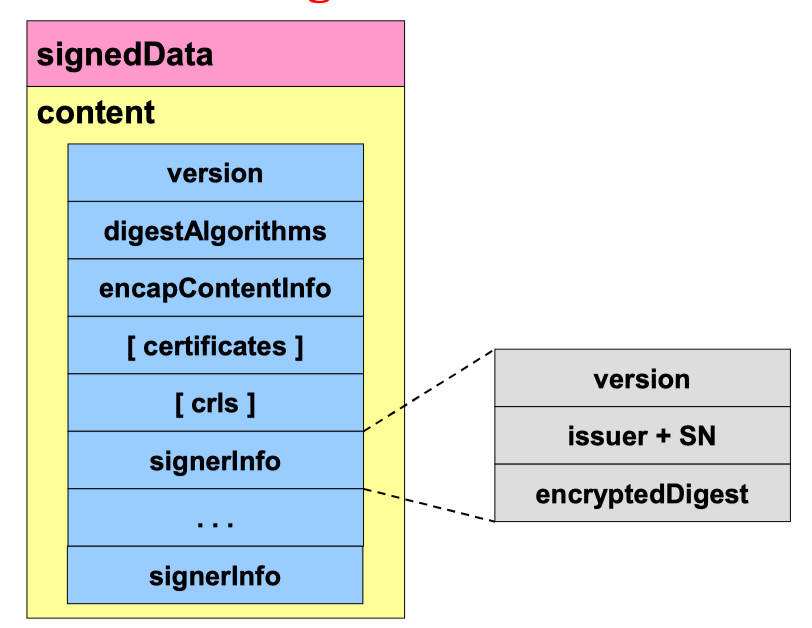
\includegraphics[width=\linewidth]{images/signedData.png}
   \caption{Signed Data}
   \label{fig:signedData}
\end{figure}
\begin{figure}[H]
   \centering
   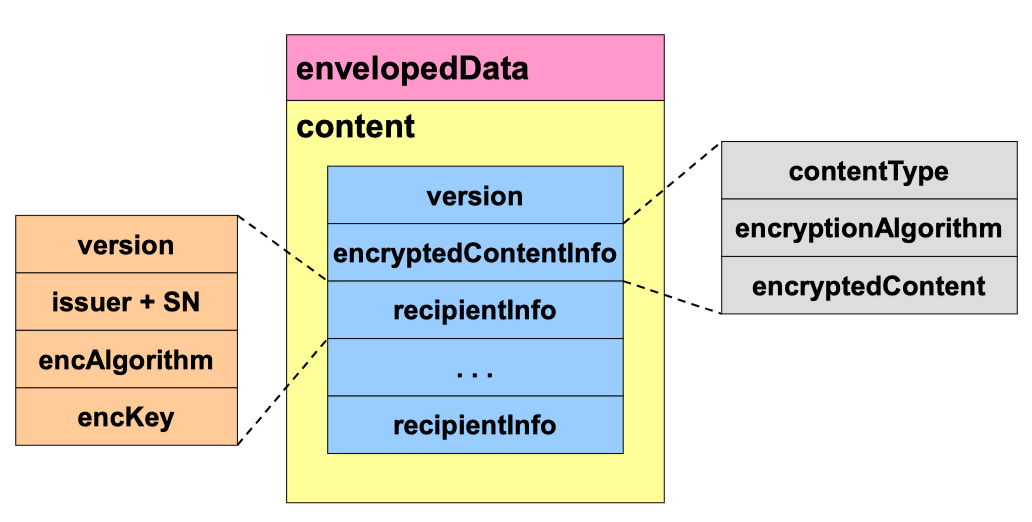
\includegraphics[width=\linewidth]{images/envelopedData.png}
   \caption{Enveloped Data}
   \label{fig:envelopedData}
\end{figure}

\subsection{PKCS\#12}
Is a standard defined by RFC for the transport of (personal) cryptographic material among applications or different system. Is used to transport a private key and one or more certificates or the digital identity of a user. Is widely used.

\subsection{Multiple Signature}
There two possible solution for multiply signing documents:
\begin{itemize}
  \item Parallel/Indipendent: Each different user sign the document indipendently, 3 digest of result. (fig. \ref{fig:parallel})
  \item Sequential/Hierarchical: Each user sign the document plus the digest of the previous signer. (fig. \ref{fig:sequential})
\end{itemize}
\begin{figure}[h!]
  \centering
  \begin{minipage}{.48\textwidth}
    \centering
    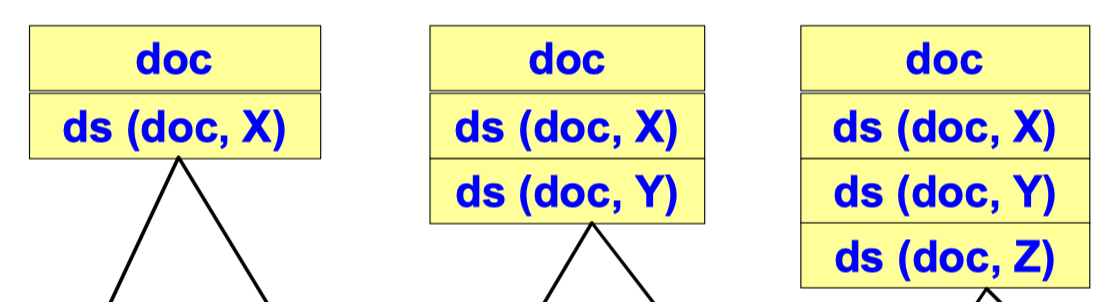
\includegraphics[width=\linewidth]{images/parallel.png}
    \caption{Parallel/Indipendent}
    \label{fig:parallel}
  \end{minipage}\hfill
  \begin{minipage}{.48\textwidth}
    \centering
    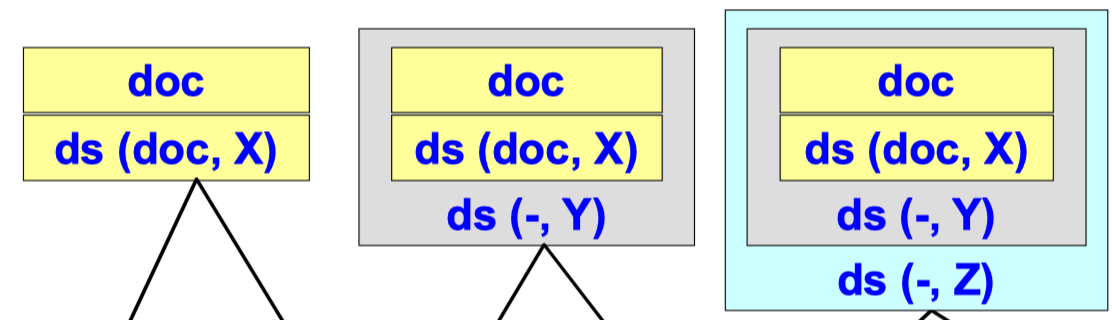
\includegraphics[width=\linewidth]{images/sequential.png}
    \caption{Sequential/Hierarchical}
    \label{fig:sequential}
  \end{minipage}\hfill
\end{figure}

\subsection{EU Eletronic Signature (ES)}
Data in electronic form which are attached to or logically associated with other eletronic data and which serve as a method of authentication. Also a scanned signature is an Electronic Signature. The goal of this solution is to provide an international standard, the difference is that is a general idea and not a technical document.\\
The \textbf{AES} (\textit{Advanced Eletronic Signature}) is a specificantion of this document. The main rules are:
\begin{itemize}
  \item Uniquely linked to the signatory
  \item Capable of identifying the signatory
  \item Created using means that the signatory can maintain under his sole control
  \item Linked to the data to which it relates in such a manner that any subsequent change of the data is detectable
\end{itemize}
The \textbf{QC} (\textit{Qualified Certificate}) is a PKC cerityfing the identity of a person and containing:
\begin{itemize}
  \item An indication that it was issued as a WC
  \item The name of the signatory or a pseudonym, which shall be identified as such
  \item Provision for a specific attribute of the signatory to included id relevant, depending on the purpose for which the certificate is intended
  \item Limitation on the scope of the certificate, if any
  \item Limits on the value of transactions, if any
\end{itemize}
The \textbf{QES} (\textit{Qualified Electronic Signature}) is an AES based on a QC, and created by a secure-signature-creation device. It satisfying the legal requirements of a signature in relation to data in eletronic form in the same manner as a handwritten signature satisfies those requirements in relation to paper-based data. Is also admissible as evidence in legal proceedings.\\
An important problem to be noticed is the "macro" problem, in general idea e-signing an e-document containing a macro is a bad idea, the verification of the data is become impossible. WYSIWYS (\textit{What You See Is What You Sign}) is highly desiderable, is a prblem of the application developers.

\section{Firewall and IDS/IPS}
\subsection{Firewall}
A firewall is a wall to protect against fire propagation, it controlls connection between networks at different security levels (boundary protection).
\begin{figure}[H]
   \centering
   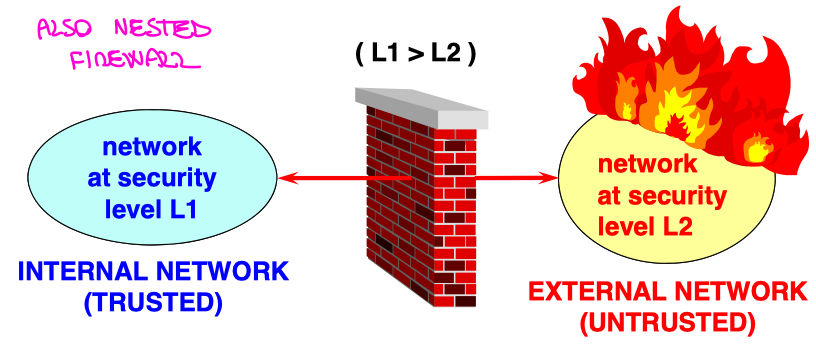
\includegraphics[width=\linewidth]{images/firewall.png}
   \caption{Firewall}
   \label{fig:firewall}
\end{figure}
There are two types of firewall:
\begin{itemize}
  \item \textbf{Ingress}: Incoming connections are managed, used to select the public services offered
  \item \textbf{Egress}: Used for check the activity of personell (Less common)
\end{itemize}
Firewall is something that can't be buyed, is designed. Of course an increased of functionality decrease se security and viceversa. There are three defined commandments for firewalls:
\begin{itemize}
  \item Thw FW must be the only contact point of the internal network with the external one
  \item Only authorized traffic can traverse the FW
  \item The FW must be a highly secure system itself
\end{itemize}
Two authorization policies can be exploited, one is the \textbf{whitelisting} where \textit{"All that is not explictly permitted, is forbidden"} that guarantee more security with an increase of difficulties to manage. The other solution, \textbf{blacklisting}, is \textit{"All that is not explictly forbidden, is permitted"} this is less secure because everything is open, but is more easy to be managed.\\
The basic options for a FW are:
\begin{itemize}
  \item Screening Router (Choke): Filters traffic at network level
  \item Bastion Host: Secure System (with Auditing)
  \item Application Gateaway (Proxy): Service that works on behalf of an application with access control
  \item Dual-homed Gateaway: System with two network cards and routing disabled
\end{itemize}
The screening router architecture exploits the router to filter the traffic both at ip and upper levels, it not require dedicated hardware, it not require a proxy and it not require modification over the application. Is simple, easy, cheap and INSECURE. (fig. \ref{fig:screening})\\
The dual-homed gateaway instead is easy to implement, require small additional hardware, it can masquared the internal network. The main problem is the is unflexible and have a large work overhead. (fig. \ref{fig:dual-homed})\\
\begin{figure}[h!]
  \centering
  \begin{minipage}{.48\textwidth}
    \centering
    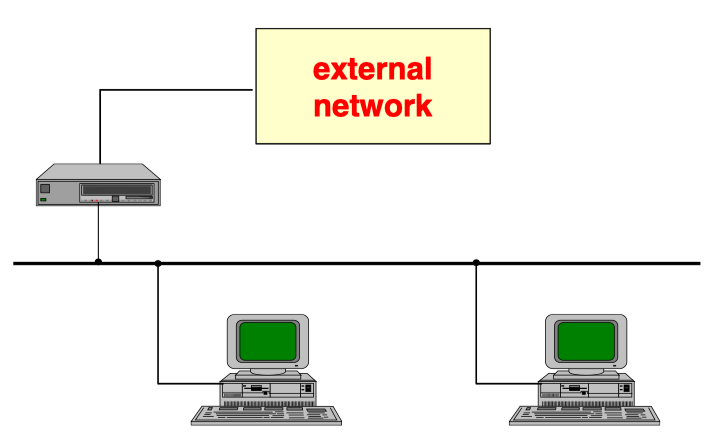
\includegraphics[width=\linewidth]{images/screening.png}
    \caption{Screening Router}
    \label{fig:screening}
  \end{minipage}\hfill
  \begin{minipage}{.48\textwidth}
    \centering
    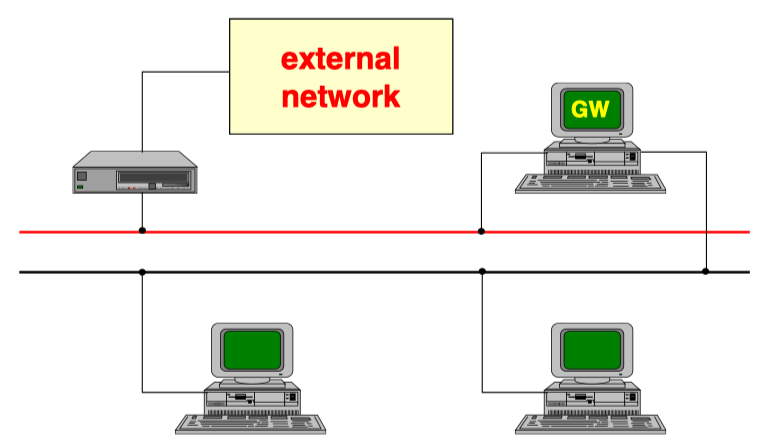
\includegraphics[width=\linewidth]{images/dual-homed.png}
    \caption{Dual-homed}
    \label{fig:dual-homed}
  \end{minipage}\hfill
\end{figure}
Another solution is the screened host (fig. \ref{fig:screened-host}), the router:
\begin{itemize}
  \item Blocks INT $\rightarrow$ EXT unless from the bastion
  \item Blocks EXT $\rightarrow$ INT unless goes to the bastion
  \item Exception: Directly enabled services
\end{itemize}
The bastion host runs cirtuit/application gateaway to control the authorized services, is more expensive and complex to manage. Is more flexible. Only the hosts/protocols passing through the bastion can be masked (unless the router uses NAT). There is also a screened subnet architecture (fig. \ref{fig:screened-subnet}), that is makes uses of the \textbf{DMZ} \textit{De-Militarized Zone}, that is a home not only to the gateway but also to other hosts, typically publis servers. The routing can be configured so that internal network is unknown. This solution is more expensive. To reduce the cost, a similar solution can be achieved with the three-legged firewall (fig. \ref{fig:3leg}).
\begin{figure}[h!]
  \centering
  \begin{minipage}{.48\textwidth}
    \centering
    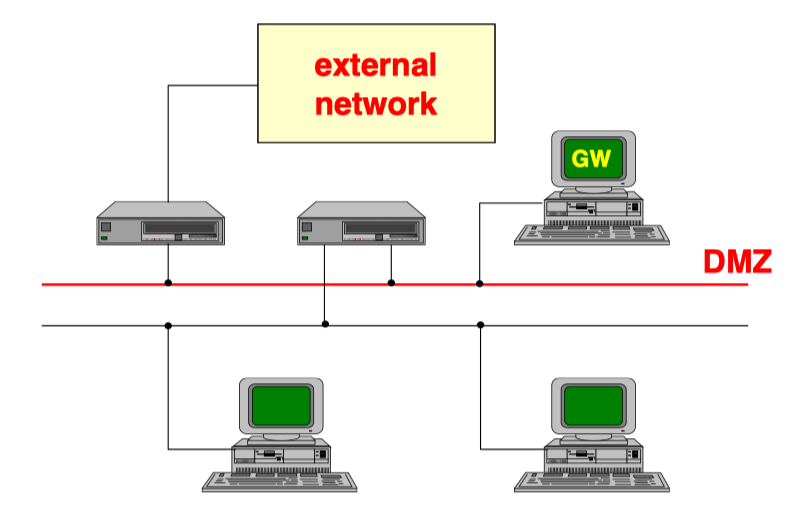
\includegraphics[width=\linewidth]{images/screened-host.png}
    \caption{Screened Host}
    \label{fig:screened-host}
  \end{minipage}\hfill
  \begin{minipage}{.48\textwidth}
    \centering
    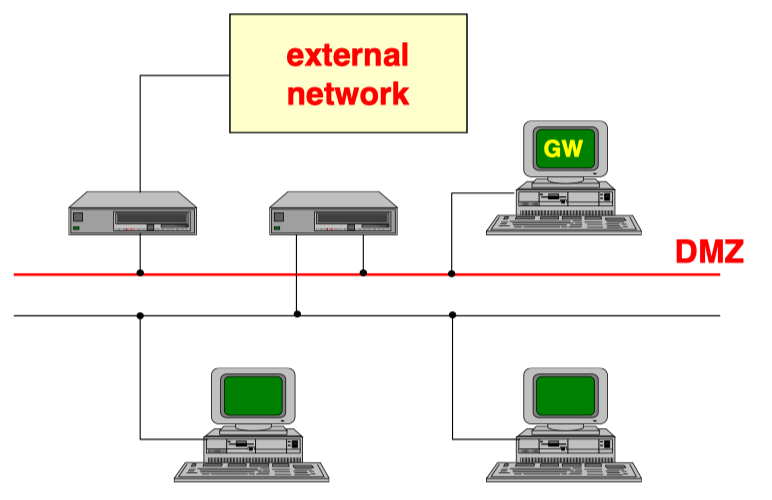
\includegraphics[width=\linewidth]{images/screened-subnet.png}
    \caption{Screened Subnet}
    \label{fig:screened-subnet}
  \end{minipage}\hfill
\end{figure}
\begin{figure}[H]
   \centering
   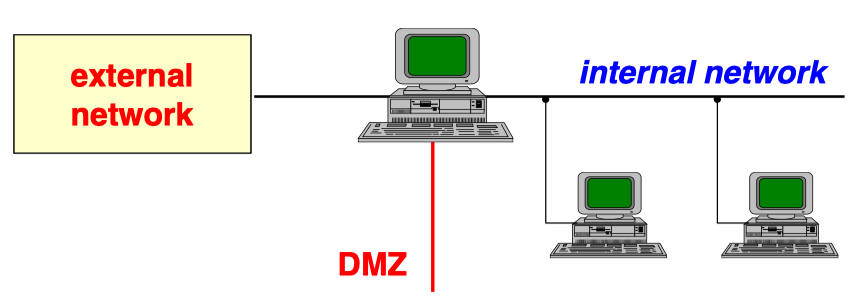
\includegraphics[width=\linewidth]{images/3leg.png}
   \caption{Three-legged Firewall}
   \label{fig:3leg}
\end{figure}

\paragraph{Techologies} There are different solutions that can be exploited to create a firewall. The difference are over perfomance, protection and over the breaking paradigm client-server.\\
The \textbf{Packet Filter} is historically available on routers and it performs packet inspection at network level, IP and transport header. THe advantages are the it scale good and makes good approximate controls. It provide good performances. It's also cheap. It has some problems with dynamically allocated ports service, it is complex to be configured and user authentication is difficult. There is also a dynamic (state-aware) version, it can distinguish from new connections from those already open it give also state informations from the transport or application level. The performance are better than the normal solution. It keep some limitations for static packet filtering.\\
The \textbf{Application-level gateway} are composed by a set of proxies inspecting the packet payload at application level. Often requires modifications to the client application, it may optionally mask the internal IP addresses, when used as part of a firewall, it performs peer authentication. It give a top security (e.g. buffer overflow of the target application). There is also a difference between forward-proxy and reverse-proxy. In this solution, the rules a more fine-grained and simpler than those of packet filter. Every application needs a spcific proxy. This solution completely breaks the client/server model, this achive more protection for the server, it may authenticate the client but is nor transparent for it. Some problem can araise with application-level security (SSL/TLS).\\
The \textbf{Circuit Level gateaway} is a generic proxy, not application-aware, it creates a transport-level circuit between client and server but it doesn; t understand or manipulate in any way the payload data. It breaks the TCP/UDP level client/server model during the connection:
\begin{itemize}
  \item More protection for server: Isolate from attacks of TCP Handshake or IP Fragementation
  \item May authenticate the client: This require modification to the application
\end{itemize}
It still exhibits many limitations of the packet filter. SOCKS is the most famous one.\\
\textbf{HTTP Forward Proxy} is an HTTP server acting just as a front-end and then passing request to the real server (external). The benefits (besides network ACL):
\begin{itemize}
  \item Shared cache of external pages for all internal users
  \item Authentication + authorization of internal users
  \item Various controls
\end{itemize}
Instead, the \textbf{HTTP Reverse Proxy} is an HTTP server acting just as a front-end for the real server(s) which the requests are passed to. The benefits (besides network ACL \& content inspection):
\begin{itemize}
  \item Obfuscation: No info about real server
  \item SSL accelerator (with unprotected back-end connections)
  \item Load balancer
  \item Web Accelerator (cache for static content)
  \item Compression
  \item Spoon Feeding (Gets from server a whole dynamic page and feed it to the client according to its speed, unload server)
\end{itemize}
The reverse proxy can be implemented in different configurations:
\begin{figure}[H]
   \centering
   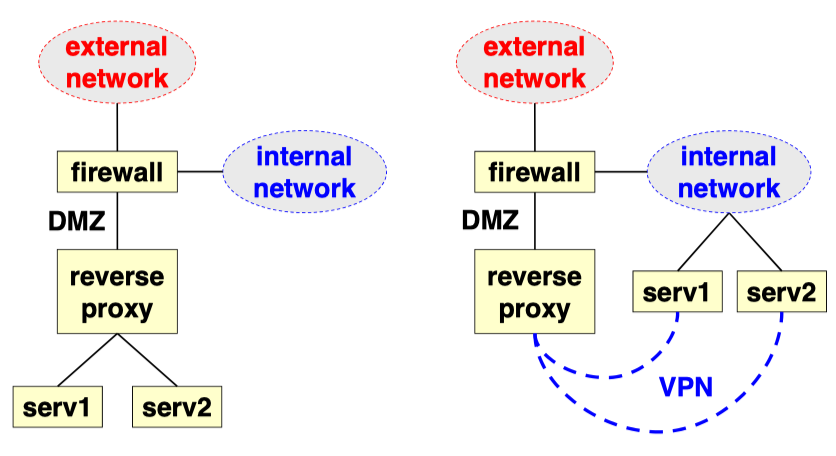
\includegraphics[width=\linewidth]{images/reverse_config.png}
   \caption{Reverse Proxy Configuration}
   \label{fig:reverse_config}
\end{figure}
The \textbf{WAF} \textit{Web Application Firewall} is really used for web application, is a module (plugin of NGINX or Apache) instead of a proxy, and is used to filter application traffic.\\
The \textbf{Stealh Firewall} is a FW without IP address, so that it cannot be directly attacked, it performs physical packet interception by setting interfaces in promiscous mode. It copies or discard network traffic without altering them.\\
There is also a local/personal version of the firewall that is directly installed at the node to be protected, is typically a packet filter. Is important to limit the diffusion of malware and trojans, or plain configuration mistakes. Of course the sys management must be separate from the firewall management.\\

A firewall is 100\% effective only for attacks over/against blocked channels, the other channels require specific protection, VPN IDS or Application level security.

\subsection{IDS: Intrusion Detection System}
A system to identify individuals using a computer or a network without authorization, also for identify authorized users violating their privileges. The basic idea is that the behavioural "pattern" is different between auth and not-auth. There are 2 types of IDS:
\begin{itemize}
  \item \textbf{Passive}: Notify after attack (Crypto checksum, pattern matching)
  \item \textbf{Active}: Notify during attack (Learn, Monitoring, Reaction)
\end{itemize}
There are also 2 topological features:
\begin{itemize}
  \item \textbf{HIDS} \textit{Host-based IDS}: Log analysis and internal OS monitoring tools
  \item \textbf{NIDS} \textit{Network-based IDS}: Network traffic monitoring tools
\end{itemize}
The \textbf{SIV} \textit{System Integrity Verifier} it checks files/filesystems looking for changes, the \textbf{LFM} \textit{Log File Monitor} checks the log files lookings for known patterns of successful attacks or attempts.\\
The NIDS is composed of 3 main parts (fig. \ref{fig:NIDS_arch}):
\begin{itemize}
  \item Sensor:
  \begin{itemize}
    \item Check traffic and logs looking for suspect patterns
    \item Generate relevant security events
    \item Interacts with the system (ACLs, TCP reset, etc...)
  \end{itemize}
  \item Director:
  \begin{itemize}
    \item Coordinates the sensors
    \item Manage the security DB
  \end{itemize}
  \item IDS Message System
  \begin{itemize}
    \item Secure and Reliable communication among the IDS components
  \end{itemize}
\end{itemize}
\begin{figure}[H]
   \centering
   \includegraphics[width=\linewidth]{images/NIDS_arch.png}
   \caption{NIDS Architecture}
   \label{fig:NIDS_arch}
\end{figure}

\subsection{IPS: Intrusion Prevention System}
To speed-up and automate the reaction to intrusions = IDS + Distributes Dynamic Firewall. This is not a product, is a technology, with large impact on many elements of the protection system. It could be dageorus and block innocent traffic. Is often integrated in a single product IDPS.

\subsection{NGFW: Next-Generation Firewall}
They can identify application, whatever network is used and, if possible, deciphering/re-chipering the traffic. Allows also user authentication and per-user or per-application policies. Another feature is the filtering based also upon know vulnabilities, threats, malware, etc...

\subsection{UTM: Unified Threat Management}
They are integration of several products in a single device (FW, VPN, IPS, IDS, etc...), the capabilities depends upon the manufacturer. An example is Sophos.

\subsection{Honey Pot}
The honey pot is a social solution to attract the attacker to some server in order to remove the interest over other more critical hosts.

\section{E-Mail Security}
The \textbf{MHS} (\textit{Message Handling System}) is the flow in charge of trasporting the mail messages. The figure below shown the flow:
\begin{figure}[H]
   \centering
   \includegraphics[width=\linewidth]{images/MHS.png}
   \caption{Message Handling System}
   \label{fig:MHS}
\end{figure}
The different part are:
\begin{itemize}
  \item \textbf{MUA}: Message User Agent
  \item \textbf{MSA}: Message Submission Agent
  \item \textbf{MTA}: Message Transfer Agent
  \item \textbf{MS}: Message Store
\end{itemize}
There are different solution for acccessing the mail system:
\begin{itemize}
  \item Client-Server Mail
  \item WebMail
\end{itemize}
\begin{figure}[h!]
  \centering
  \begin{minipage}{.48\textwidth}
    \centering
    \includegraphics[width=\linewidth]{images/cs_mail.png}
    \caption{Client-Server}
    \label{fig:cs_mail}
  \end{minipage}\hfill
  \begin{minipage}{.48\textwidth}
    \centering
    \includegraphics[width=\linewidth]{images/webmail.png}
    \caption{WebMail}
    \label{fig:webmail}
  \end{minipage}\hfill
\end{figure}
The main standard for the exchange are:
\begin{itemize}
  \item \textbf{SMTP}: Simple Mail Transfer Protocol [TCP@25 - TCP@587]
  \item \textbf{POP}: Post Office Protocol [TCP@110]
  \item \textbf{IMAP}: Internet Message Acces Protocol [TCP@143]
\end{itemize}
The message standard was defined in the RFC-822, it use only US-ASCII characters on 7 bits, the line are terminated by CR+LF and is composed by header + body. The header is composed of multiple fields:
\begin{itemize}
  \item From (logical) - Sender (operational)
  \item Organization
  \item To
  \item Subject
  \item Date
  \item Received (Intermediate Steps)
  \item Message-Id (sending ID)
  \item CC - BCC (Copy to)
  \item Return-Receipt-To
\end{itemize}
The main problems of the mail are: Connectionless system (store and forward), the untrusted MTA, the security of MS, the mailing-list encryption and the compatibility with what is already installed.\\

\subsection{Spamming}
One of the most known problems of the mail is the spamming, also know as \textbf{UBE} \textit{Unsolicited Bulk Email} or \textbf{UCE} \textit{Unsolicited Commercial Email}, is the sending of unwanted messages: unauthorised advertisement, attacks like malware and phising and so on. Today is nearly the 88\% of the toal email traffic, this means heavy load on servers and network channels and also annoyance to the users. The opposite of the spam is the ham.\\
\paragraph{Spamming strategies} are hiding the real sender, but using a valid sender, they are using special MTA with open mail relay (MTA that accept mail also not from/to its users), zombies or botnet and they are using content obfuscation to pass the filtering.\\
A good anti-spam solution for MSA is to not configure your own MSA as an "open relay", but restrict its use only to authorized users. Is also important to authenticate the users of our MSA:
\begin{itemize}
  \item IP Address of MUA
  \item Value of the filed FROM
  \item SMTP authentication
\end{itemize}
Also reject or accept mail from an MTA, after checking a blacklist or whitelist like the DNS-based Blacklist. Another solution is the DNS-Blacklist by URI reputation, it has some problem to deteching new spammer, but is a good solution with honey pot.\\
The most important \textbf{DNSBL} lists are:
\begin{itemize}
  \item MAPS RBL (Realtime Blackhole List)
  \item Spamhaus SBL
  \item SORBS (Spam and OpenRelay Blocking System)
  \item APEWS (Anonymous Postmaster Early Warning System)
\end{itemize}
Exiting from this lists is not easy once inserted. Using \textbf{greylisting} will "temporarily reject" any email from a sender it does not recognize. If the mail is legitimate, the originating server will try again after a delay, and if sufficient time has elapsed, the email will be accepted. The main drawback is the delay of ham and the increase of server load.\\
Other technique is the \textbf{DKIM} (\textit{Domain Keys Identified Mail}), a mail domain guarantee (via DS) the identity of the sender and the partial integrity of the message, the DS is created by the MSA or outgoing MTA, which covers some headers and part of the body and is verifiable via a public key.

\subsection{Protocols}
\paragraph{DMARC} is the (\textit{Domain-based Message Authentication, Reporting and Conformance}), used by service like Google, Yahoo!, PayPal and so on. Is based on some high levels principles:
\begin{itemize}
  \item Senders clearly opt-in by pushing DMARC policy
  \item Receivers provide feedback so senders can close gaps
  \item Senders increase level of authenticated email
  \item Receivers can identify and block unauthenticated email
\end{itemize}
Is build up DKIM and SPF, DKIM signature may work when a SPF path doesn't, SPF may work even if the sender screws up DKIM temporarily.
It allows policy assertions to quarantine or block messages that do not authenticate. Collects also a lot of data for reporting. It improves over DKIM/SPF, some problems remain with indirect mails.

\paragraph{ESMTP} is the extended version of SMTP, the base protocol and the communication channel is the same. The ESMTP clients must identify themselves to the communicating parties with: EHLO \textit{hostname}, if the server understands ESMTP it must declare the extensions that it supports, one per line, in its response to EHLO.\\
The SMTP-auth is an another extension of ESMTP, it provides the AUTH command, plus some options of MAIL FROM, to authenticate a client before accepting messages from it. This solutions is useful against spamming.\\
The auth can be of two types:
\begin{itemize}
  \item PLAIN: by passing the pwd and the id over a base64 (not ciphered)
  \item CHALLENGE: by completing a challeng in order to verify identities
\end{itemize}
The challenge could be performed in two ways:
\begin{itemize}
  \item CRAM-MD5
  \item DIGEST-MD5 (now replaced by SCRAM)
\end{itemize}
The first solution have some advantages: client auth via password, no replay and secure to sniffing. The main drawbacks are: no server authentication, cleartext storage of pwd, vulnerable to dictionary attacks, possible MITM.\\
\textbf{SCRAM} instead is a Salted Challenge-Response Authentication Method, this methods allows a mutual authentication, difficult attacks against pwd in DB, is easier to be implemented and the standard encoding is UTF-8. SCRAM can be extended via \textbf{CB} (\textit{Channel Binding}) it associate a secure channel (typically encrypted) with an application exchange providing mutual authentication to avoid a MITM as end-point for the encrypted channel which the intercepts the application data. There are two main classes:
\begin{itemize}
  \item Unique: Specific channel
  \item End-point: Same channel for secure and application
\end{itemize}
The supported methods are based on SCRAM-SHA-1 and SCRAM-SHA-1-PLUS with the CB mode.

\paragraph{SMTP+TLS} is the SMTP service extensione for SMTP over TLS, the option of EHLO is \textbf{STARTTLS}. If the negotiation of EHLO is succesful, the protocol status is reset (start again from EHLO and the extensions supported can be different). In case of insufficent security level, the client quit immediately and close the connection and the server responds to each command with code 554 (low security).

\subsection{Security Services}
The main security services are:
\begin{itemize}
  \item Integrity
  \item Authentication: Identifies sender
  \item Non repudiation
  \item Confidentiality
\end{itemize}

\end{document}
